\documentclass[10pt,a4paper]{article}

\usepackage{graphicx}
\usepackage{verbatim}
\usepackage{subcaption}
\usepackage{amssymb}
\usepackage{pifont}
\usepackage{geometry}
\usepackage{hyperref}
\usepackage{amsmath}
\usepackage{lineno}

\begin{document}
\linenumbers

\section{Hit and Track Finding}\label{sec:hitstracks}

The BHF is an algorithm that does both hit reconstruction and 2D track reconstruction using collection plane hits and muon counter information, and is used in the electron lifetime analysis. The first step is to apply stuck ADC mitigation and pedestal subtraction on the collection wire raw waveforms. Then, channel-by-channel, the waveform is copied to two parallel paths, $A$ and $B$, for processing. Path $A$ begins with the application of a single-pole recursive filter with 6 sample decay time (-3~dB cutoff frequency of 53~kHz)~\cite{dsp-book} both forwards and backwards in the time domain to preserve the peak timing of the pulses. To reduce the impact of signal on the noise measurement, the waveform noise RMS is calculated as the median of the RMSs of all possible consecutive spans of 50 ticks in the waveform. Following this, unipolar pulses are found when the amplitude of the filtered waveform raises above twice the measured noise RMS value. In addition to pulses created by real charge deposits, the low threshold causes many pulses to be found which do not correspond to any real particle track or shower. The start and end points of the pulse are fixed at -50 and +100 ticks, respectively, in relation to the first tick at which the pulse raises above threshold. This 150 tick pulse width was chosen to be wide enough to fully account for the variations in true width due to different track angles with respect to the collection plane, for the triggered tracks. After all pulses on each waveform are detected, all combinations of pulses which have overlapping end and start values are merged. Each resulting pulse is denoted as a ``hit'', and has a set of calculated parameters. The peak tick of the hit is calculated as the weighted mean tick between the start and end of the pulse. In this calculation, the weight function for tick $i$ is $w_i = \exp\left[(a_i-\sigma)/\sigma\right]$, where $a_i$ is the ADC value of tick $i$, and $\sigma$ is the waveform noise RMS. This weighting scheme was chosen to avoid negative weights and to overcome biases to the peak tick by the asymmetric fixed start and end ticks for each hit. The drift time for the hit is calculated as the peak time minus the muon counter trigger time. The hit charge is calculated by integrating the ADC values of the unfiltered waveform in path $B$ between the start and end times as determined from the filtered waveform in path $A$. Hit $x$ coordinates are determined using the drift time and the electron drift velocity, and the $z$ coordinates are simply the $z$ location of the wire. The $y$ coordinate of each hit was not measured directly as induction plane signals were not analysed, but could be roughly inferred through interpolation given the triggered muon counter $x$, $y$, and $z$ locations.

The THB algorithm was developed to purify the hits collection output of the BHF and to recover charge signals which were missed because they were below the hit finding threshold. The THB begins by masking out BHF hits which are further than 25~cm distance from the line which connects the two triggered muon counters in $x-z$ space. The hits that pass this cut are subject to a robust polynomial fitting process, based on the MLESAC algorithm~\cite{MLESAC}. The algorithm fits a subsample of the event hits to a quadratic polynomial model (small curvatures are allowed in the track to account for the effects of field non-uniformities on drifting charge caused by space charge, as well as multiple coulomb scattering), then calculates the negative log likelihood which weights hits within a threshold distance of the best-fit model based on this distance, and weights outliers zero. The process is repeated over many subsamples of hits until the minimum negative log likelihood is found within a fixed number of iterations. The final step in the THB is to overlay the track in wire-time space onto all of the collection plane waveforms. If the wire signal did not raise above the hit finding threshold in the BHF on any non-bad wire at the time where the track predicts a hit should exist, a charge deposit is assumed at that time and location. For these assumed hits, the start and end times are interpolated using hits found by the BHF on neighbouring wires, and the hit peak time and charge are calculated in exactly the same way as the hits found in the BHF. A pseudo-3D reconstruction of the track in the detector is created by using the $z$ and $x$ coordinates of the hits, and roughly estimating the $y$ coordinate by using the triggered muon counter locations. The track angles with respect to the anode plane are also estimated by using the 3D line which connects the centers of the triggered muon counters.

\section{Electron Lifetime Measurement}\label{sec:lifetime}

Free electrons in the LAr attach to electronegative impurities (such as oxygen and water), reducing their drift velocity so they no longer contribute to hits, thereby reducing the total charge collected at the anode. The electron lifetime, $\tau$, is defined by the exponential decay of the collected charge at the anode, $Q_{\rm{c}}$, with drift time, $t$, 
\begin{equation}\label{eq:lifetime}
Q_{\rm{c}} = Q_{0} e^{-t/\tau},
\end{equation}
where $Q_{0}$ is the charge liberated in the ionization after recombination. For example, a reduction of charge collected of $Q_{\rm{c}}/Q_{0}\approx 51\%$ is expected for a drift of 2.2~m, an electric field of 250~V$\!$/cm, and an electron lifetime of 3~ms. Such a measurement is important in quantifying and correcting for the overall effect of impurities inside the TPC on the drifting ionization charge. Therefore, measuring the electron lifetime with a high accuracy is a required calibration task for the next generation of massive liquid argon TPCs.

Complementary to the dedicated purity monitors, the electron lifetime of the liquid argon was studied using cosmic ray muon tracks in the TPC. Several experiments have successfully measured the electron lifetime using methods similar to the one described here \cite{lifetimeT600, lifetime120L, lifetimeT600_again,lifetime-argoneut,lifetime-longbo}.

In this analysis, hits associated with successfully reconstructed tracks from the THB (section~\ref{sec:hitstracks}) are used to determine the lifetime. The collected hit charge on the readout wires follows a Landau distribution, and the electron lifetime is determined by the decrease in the most probable value (MPV) of the distribution as a function of drift time. To account for varying track angles with respect to the anode plane, the hit charge on each wire is divided by the factor $d/\cos{\theta}$ where $d$ is the collection wire spacing and $\theta$ is the angle between the track and the vector perpendicular to the collection wire and in the plane of wires. The resulting set of normalized hit charges ($dQ/dx$) are divided into 22 drift time bins, each of width $\sim$91.5~$\mu$s ($\sim$10~cm given the drift velocity) based on the hit drift times as calculated by the BHF (section~\ref{sec:hitstracks}). Three examples of bins of $dQ/dx$ are shown in figure~\ref{fig:dqdx_examples}, along with equivalent distributions for the simulated sample and MC truth, which are described in section~\ref{sec:lifetimebias}. In each bin, Minuit is used to fit a Landau convoluted with a Gaussian to the data. The range for these fits is truncated to exclude contributions from delta rays, which improves the resolution on the MPV of the fit. The extracted Landau MPVs from the fits, along with the fit errors on the MPV parameter, are then plotted against mean drift time for the bin, and the raw exponential lifetime, $\tau_{\rm{raw}}$, determined from a fit. 

\begin{figure}
\centering
\begin{subfigure}{0.33\linewidth}
\centering
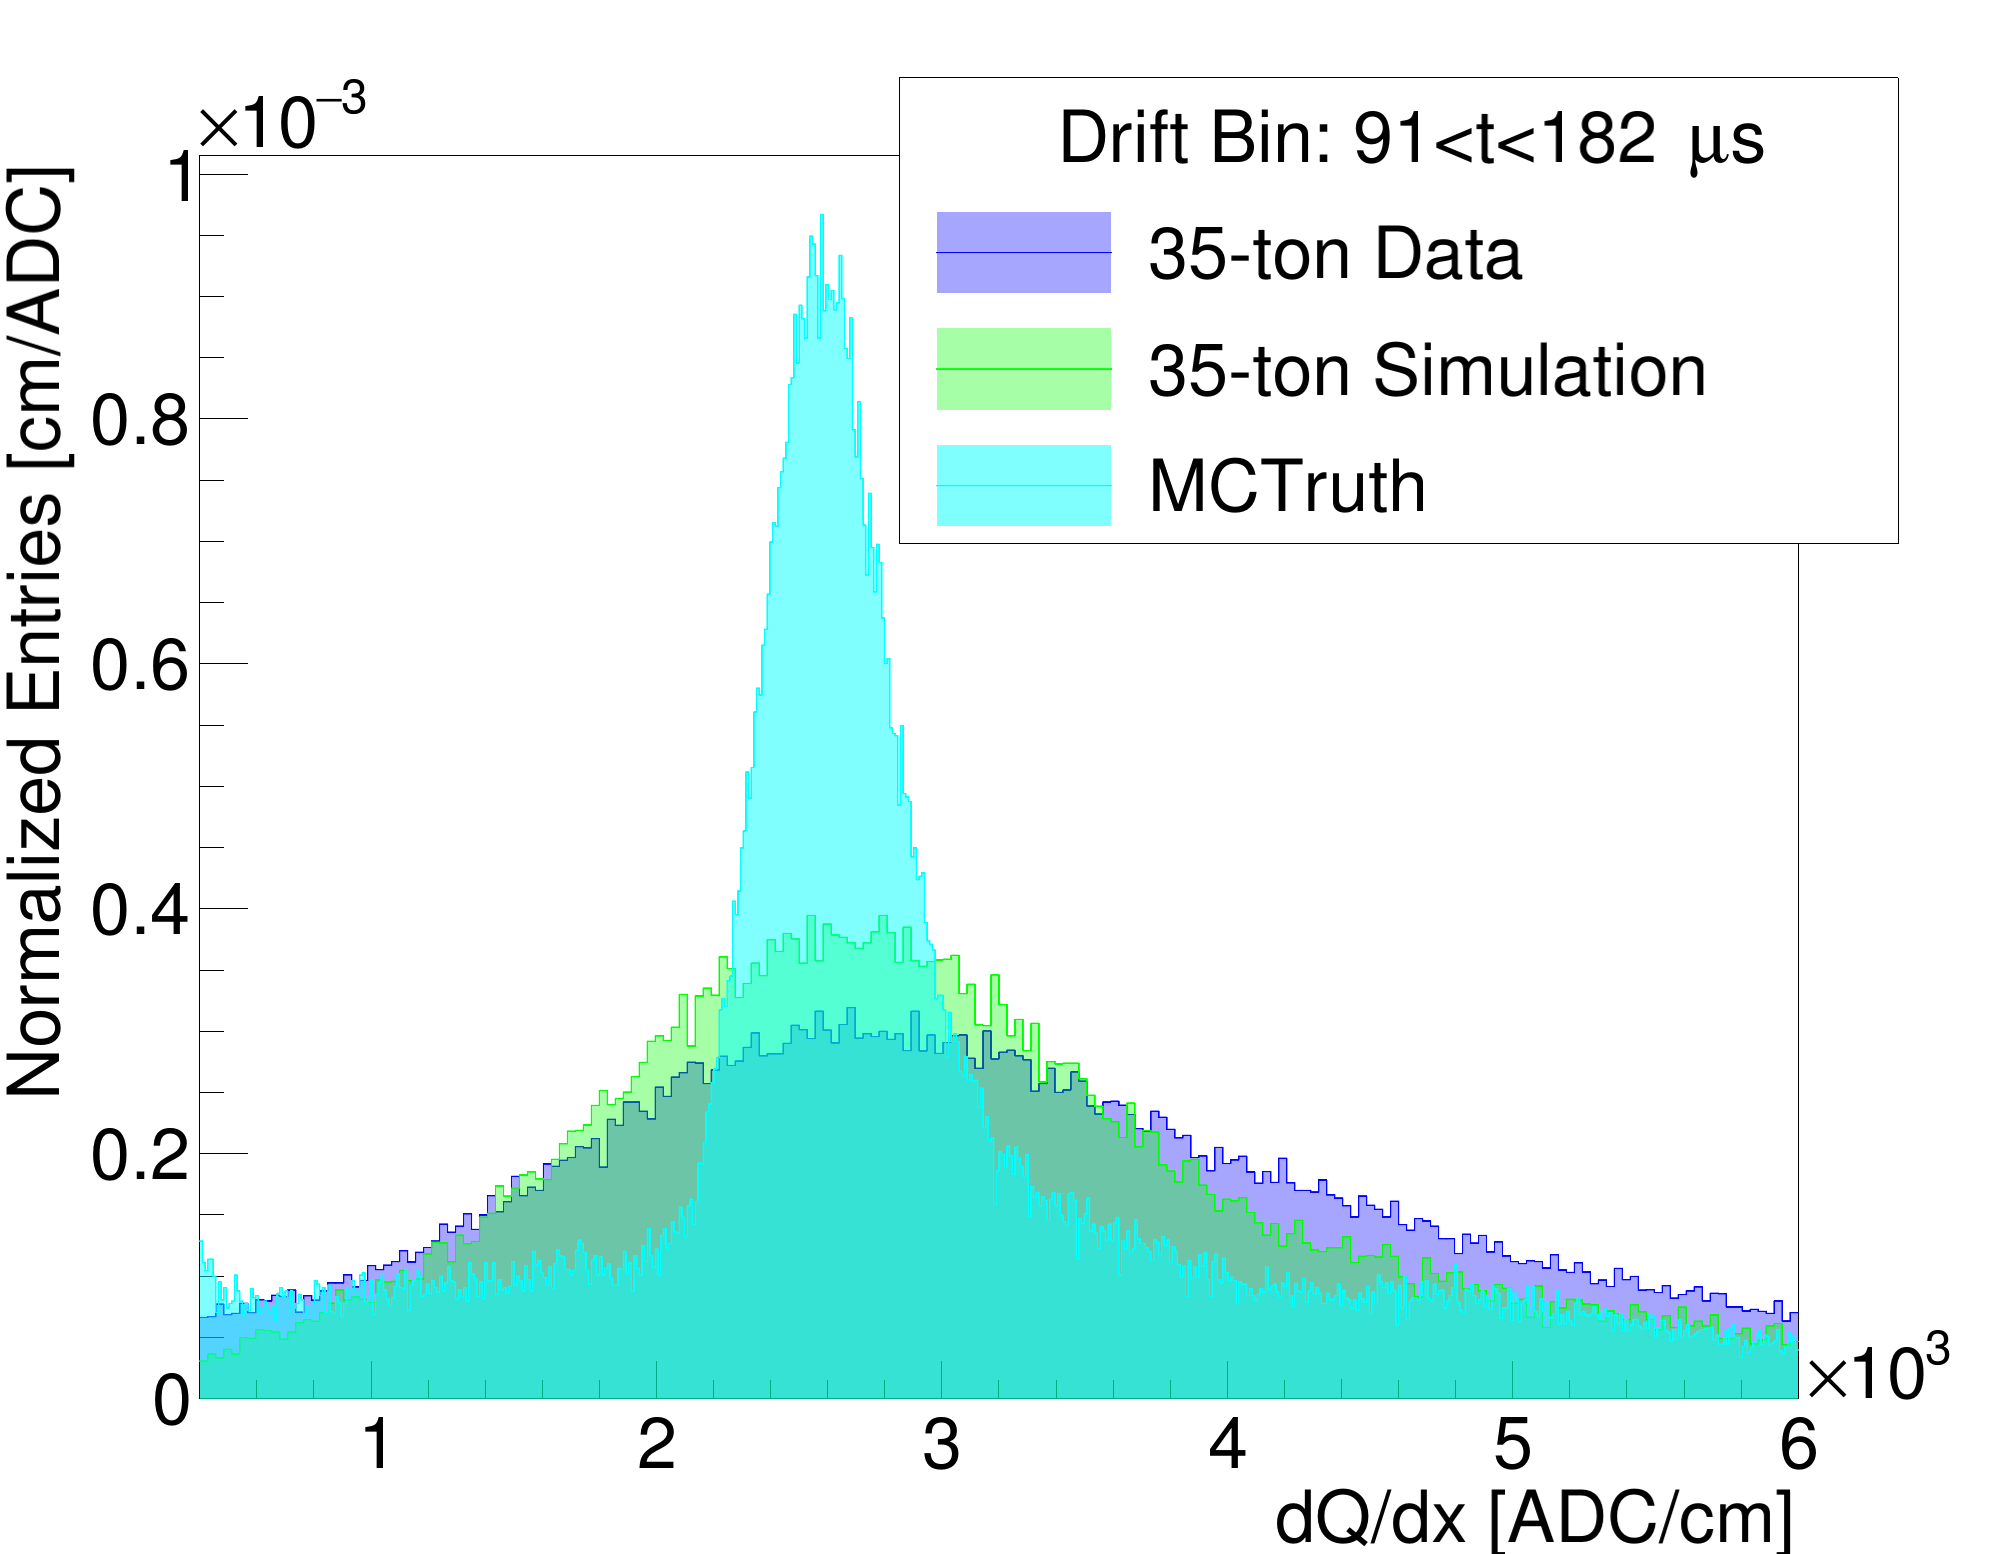
\includegraphics[width=\textwidth]{short_dqdx.png}
\caption{Short Drift\\ ($91< t_{drift}< 182$ $\mu$s)}
\label{fig:short_dqdx}
\end{subfigure}\hfill
\begin{subfigure}{0.33\linewidth}
\centering
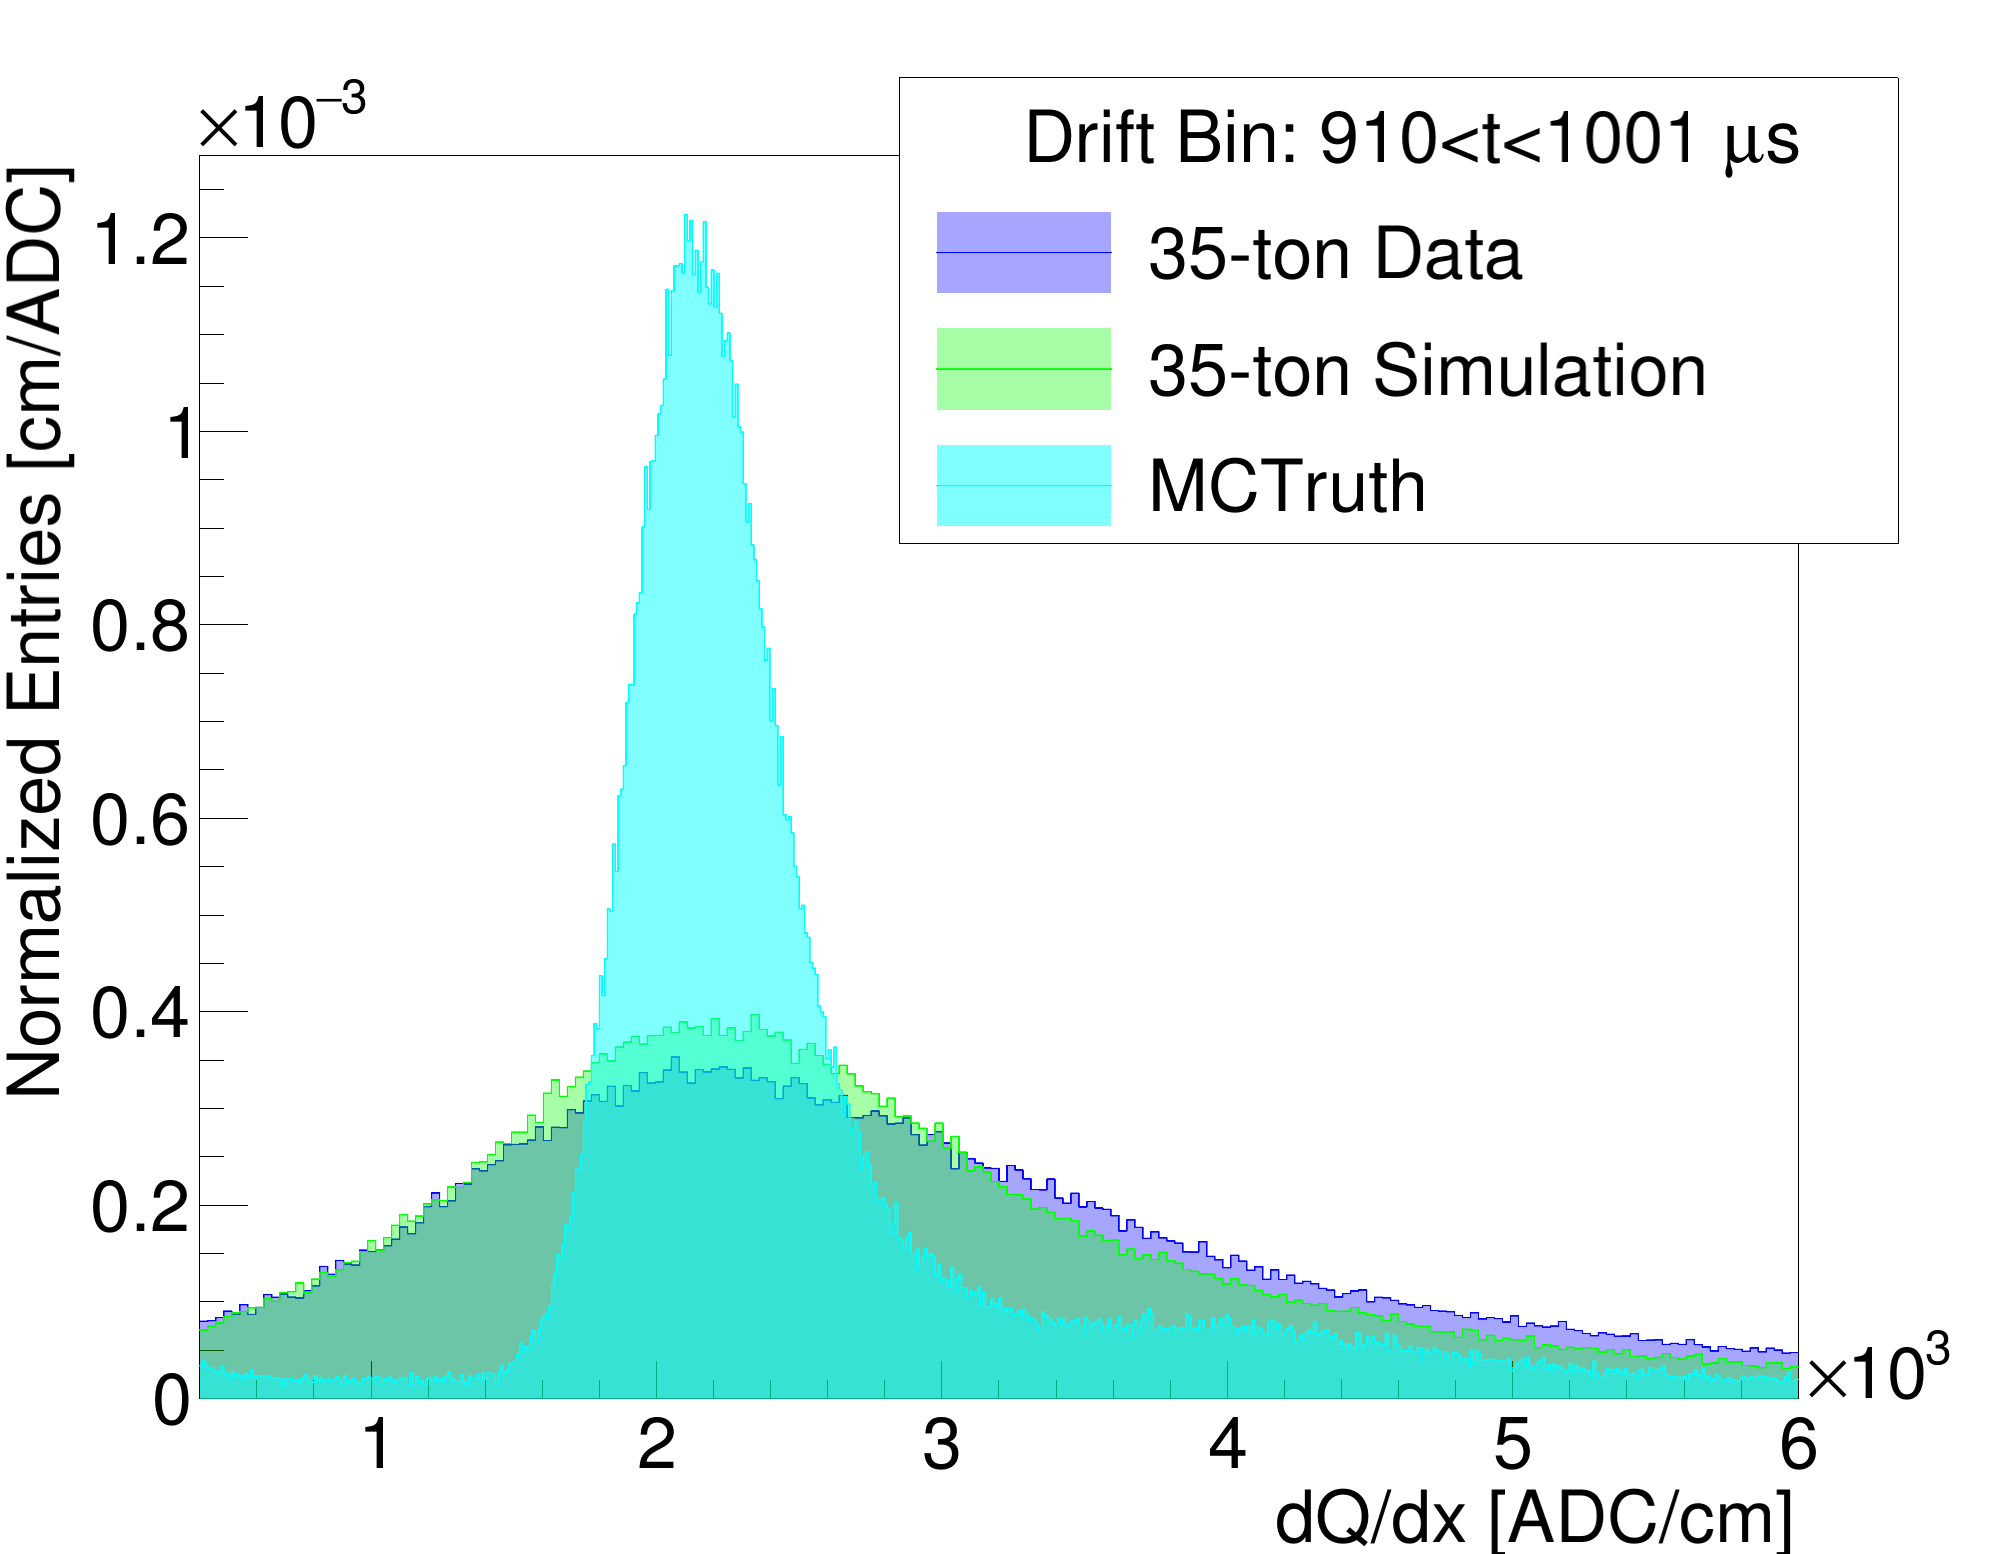
\includegraphics[width=\textwidth]{middle_dqdx.png}
\caption{Medium Drift\\ ($910<t_{drift}<1001$ $\mu$s)}
\label{fig:middle_dqdx}
\end{subfigure}\hfill
\begin{subfigure}{0.33\linewidth}
\centering
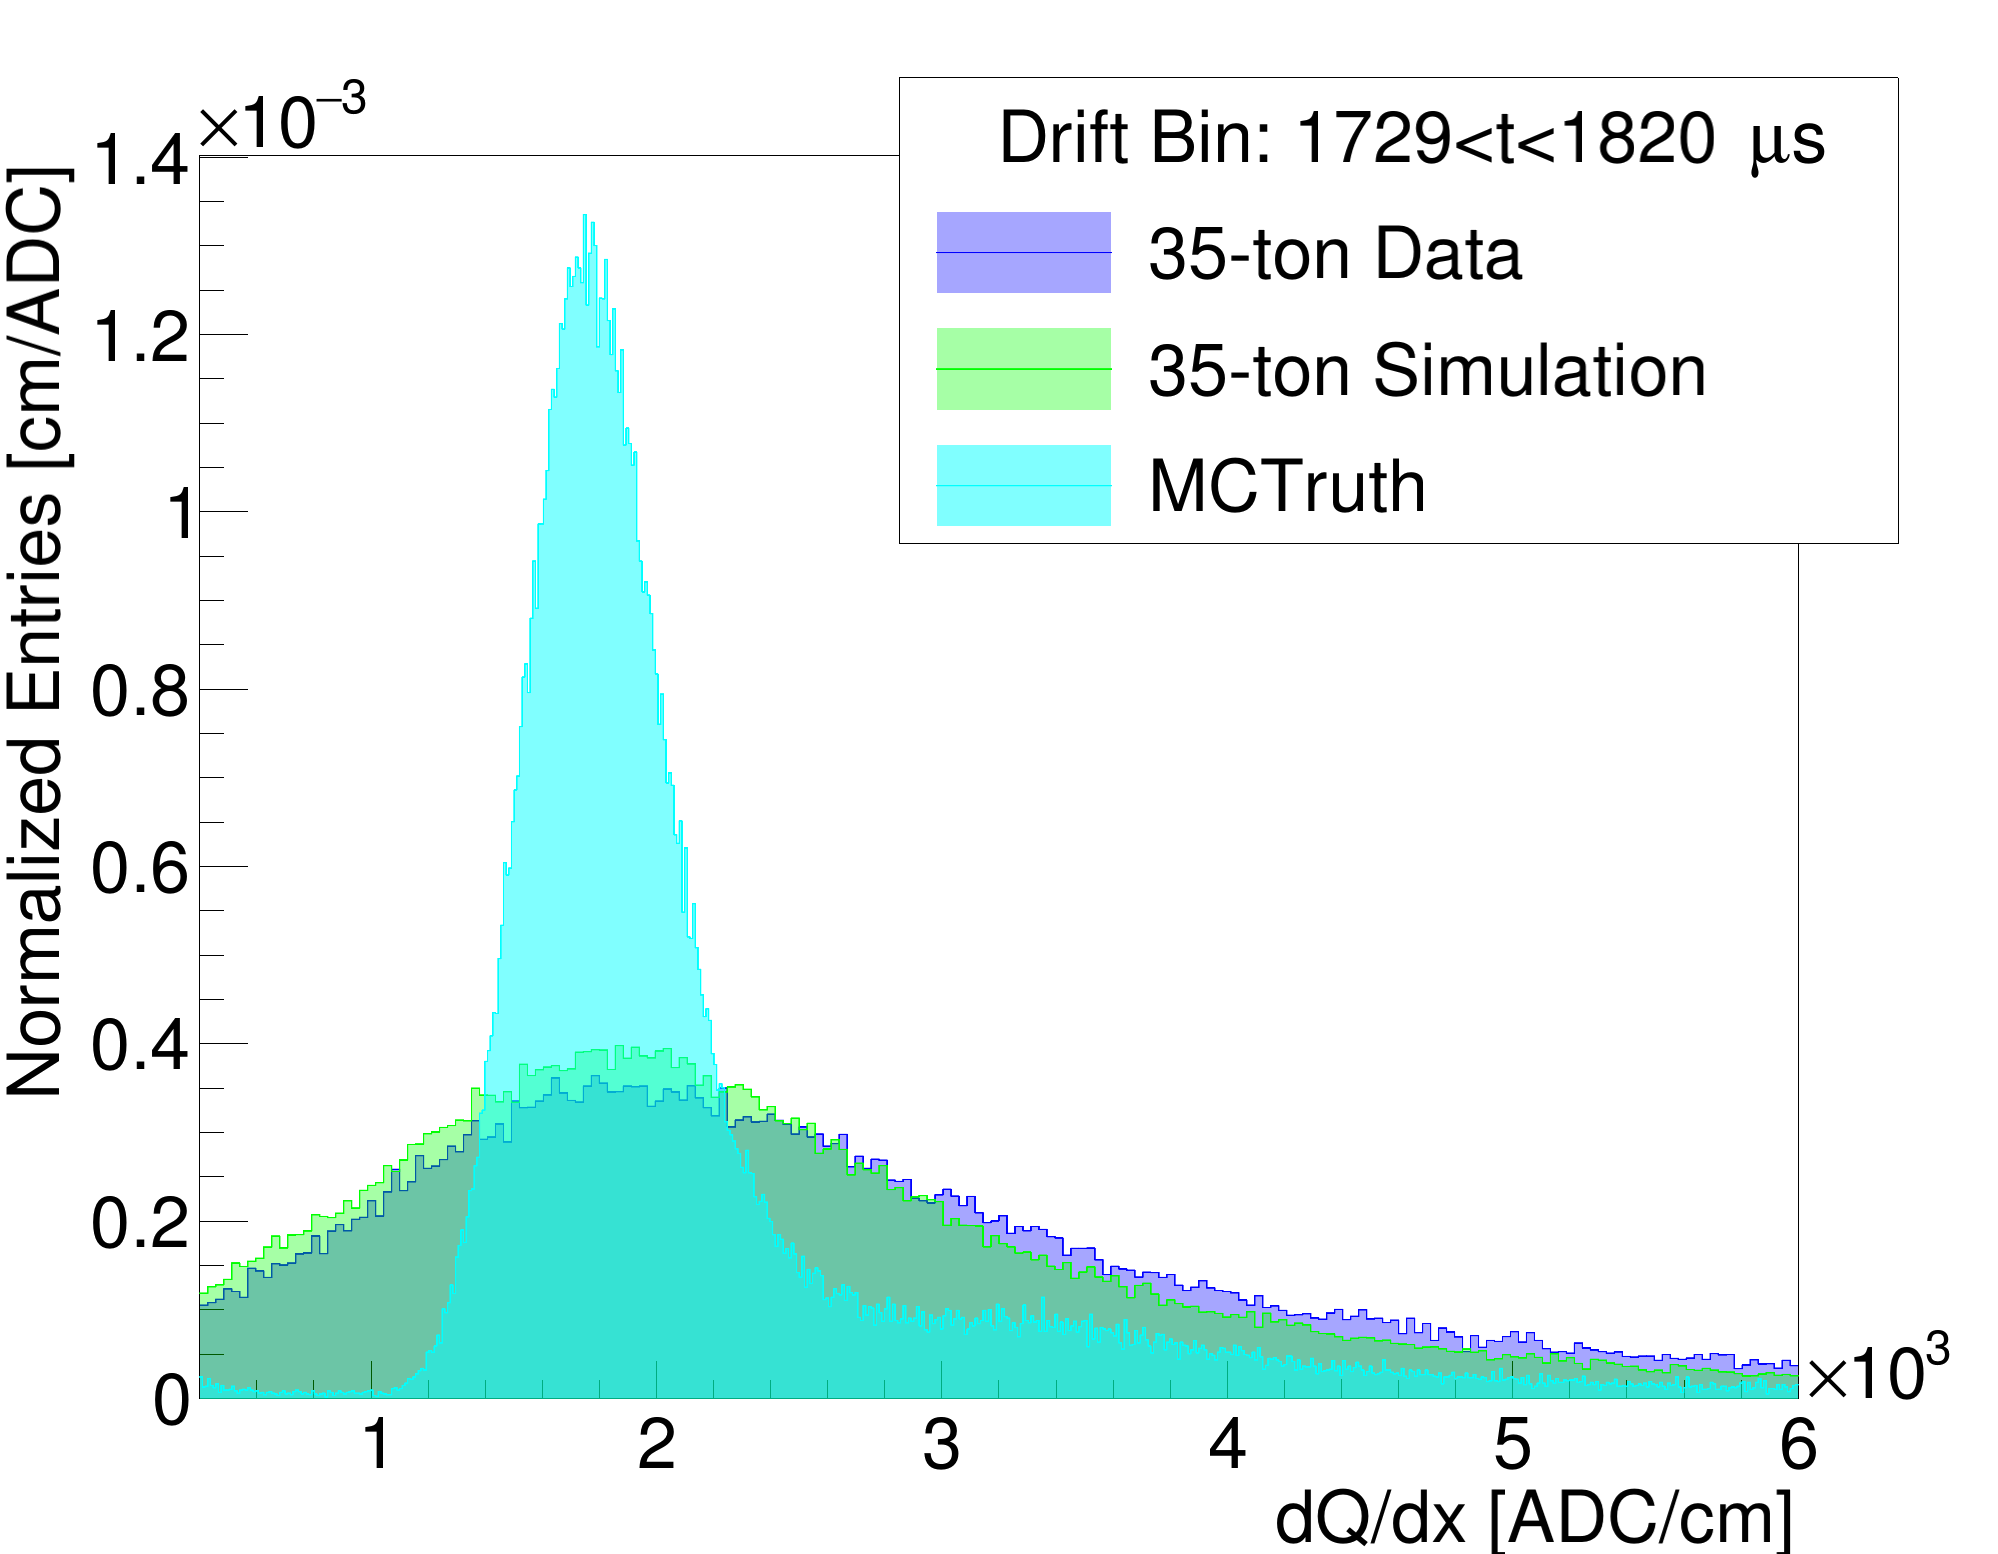
\includegraphics[width=\textwidth]{long_dqdx.png}
\caption{Long Drift\\ ($1729<t_{drift}<1820$ $\mu$s)}
\label{fig:long_dqdx}
\end{subfigure}
\caption{$dQ/dx$ from reconstructed 35-ton data, simulation, and MC truth. Simulation uses $\mu=1.153$ and $\tau_{MC}=4000\ \mu$s.}
\label{fig:dqdx_examples}
\end{figure}

The data used in this analysis consists of 17,490 events, triggered on East-West crossing muons, from five consecutive days of the Phase~II run when the cathode HV was stable, the PrMs reported greater than 2~ms lifetime, and the detector was in the low noise state. Fluctuations in the electron lifetime over the course of the dataset are not studied in this analysis, but are measured by the PrMs. They vary by approximately 4\% over the course of this dataset. As measured by PrM2, the mean lifetime in the cryostat but outside of the TPC for this dataset is $2.8\pm0.1$~(stat.)~$\pm0.5$~(syst.)~ms, as in figure~\ref{fig:PrM2}. 

\begin{figure}
\centering
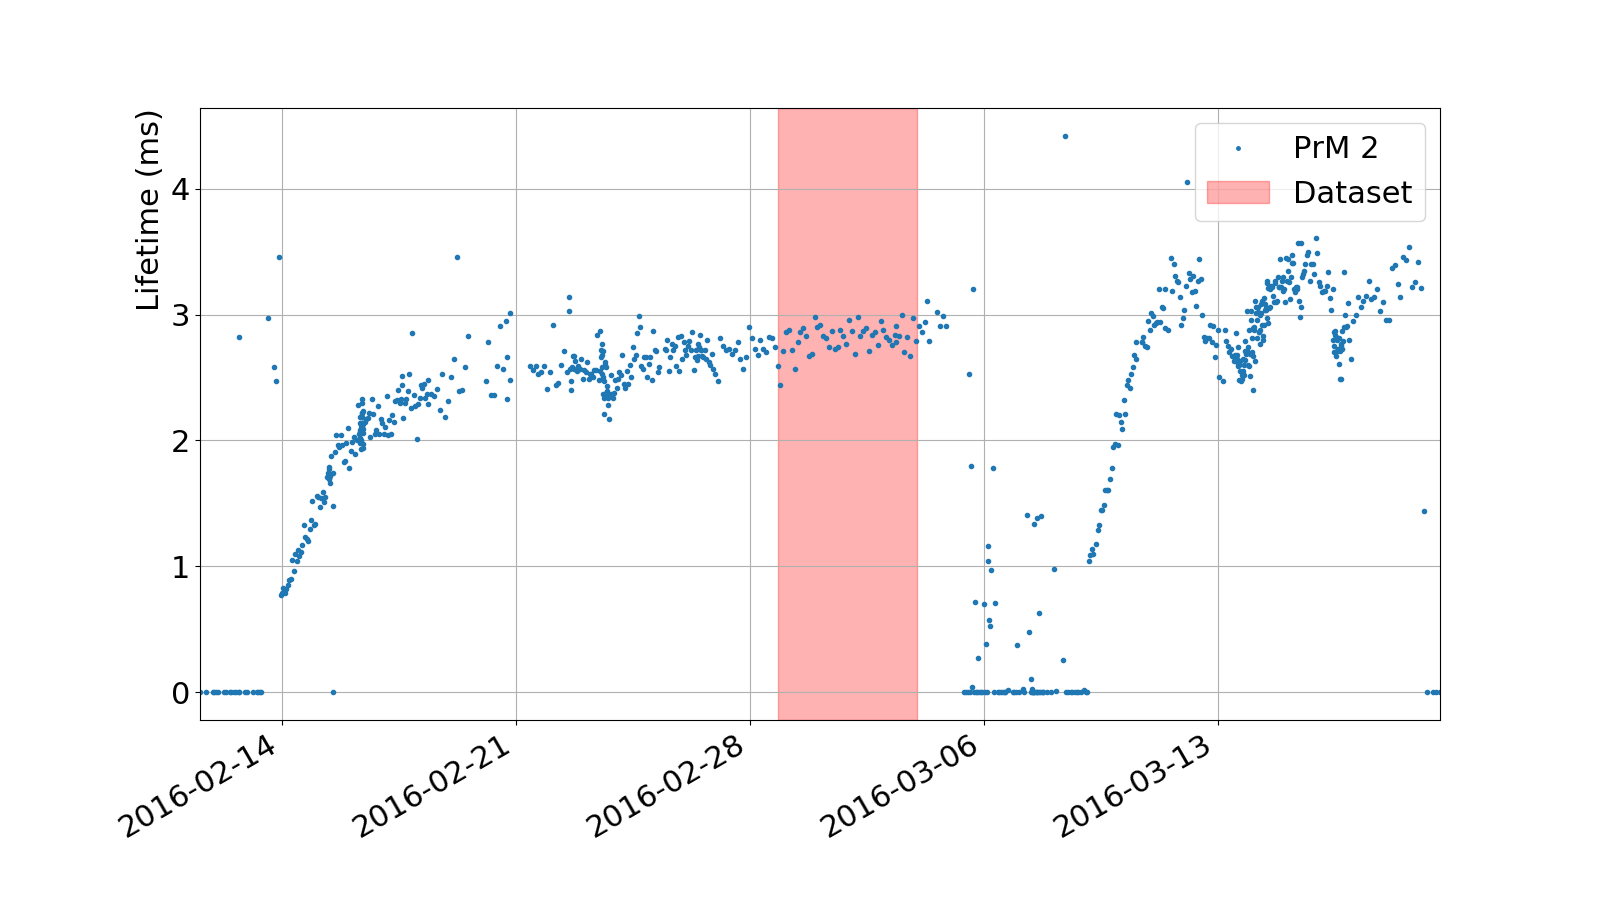
\includegraphics[width=0.8\textwidth]{PrM2.png}
\caption{PrM 2 measured electron lifetimes over the course of the 35-ton Phase II run. The times during which the data in this analysis were recorded are shown in shaded red regions.}
\label{fig:PrM2}
\end{figure}

For this dataset, the decrease of MPV $dQ/dx$ as a function of drift time in the TPC is shown in figure~\ref{fig:landMPV}, yielding an observed raw exponential lifetime of $\tau_{\rm{raw}}=4.24\pm0.10$~(stat.)~ms. The fit is done using the TMinuit class in ROOT, and has a minimum $\chi^2$/N.D.F. of 6.0. Here, a fiducial cut of 5-50\% of the full drift time is imposed to reduce bias due to incorrectly and imprecisely determined MPV for longer drift hits as well as timing offsets (explanation in section~\ref{sec:fiducialcut}). In addition, the first bin is ignored from the fit due to possible biases in the charge distributions of tracks near the anode with hit times close to the trigger time, and as a result of charge deposited within the wire planes (see section~[TODO: reference Mike's T0 stuff]). Possible additional causes of bias in this measurement and explanation of the systematic uncertainties are described below.

\begin{figure}
\centering
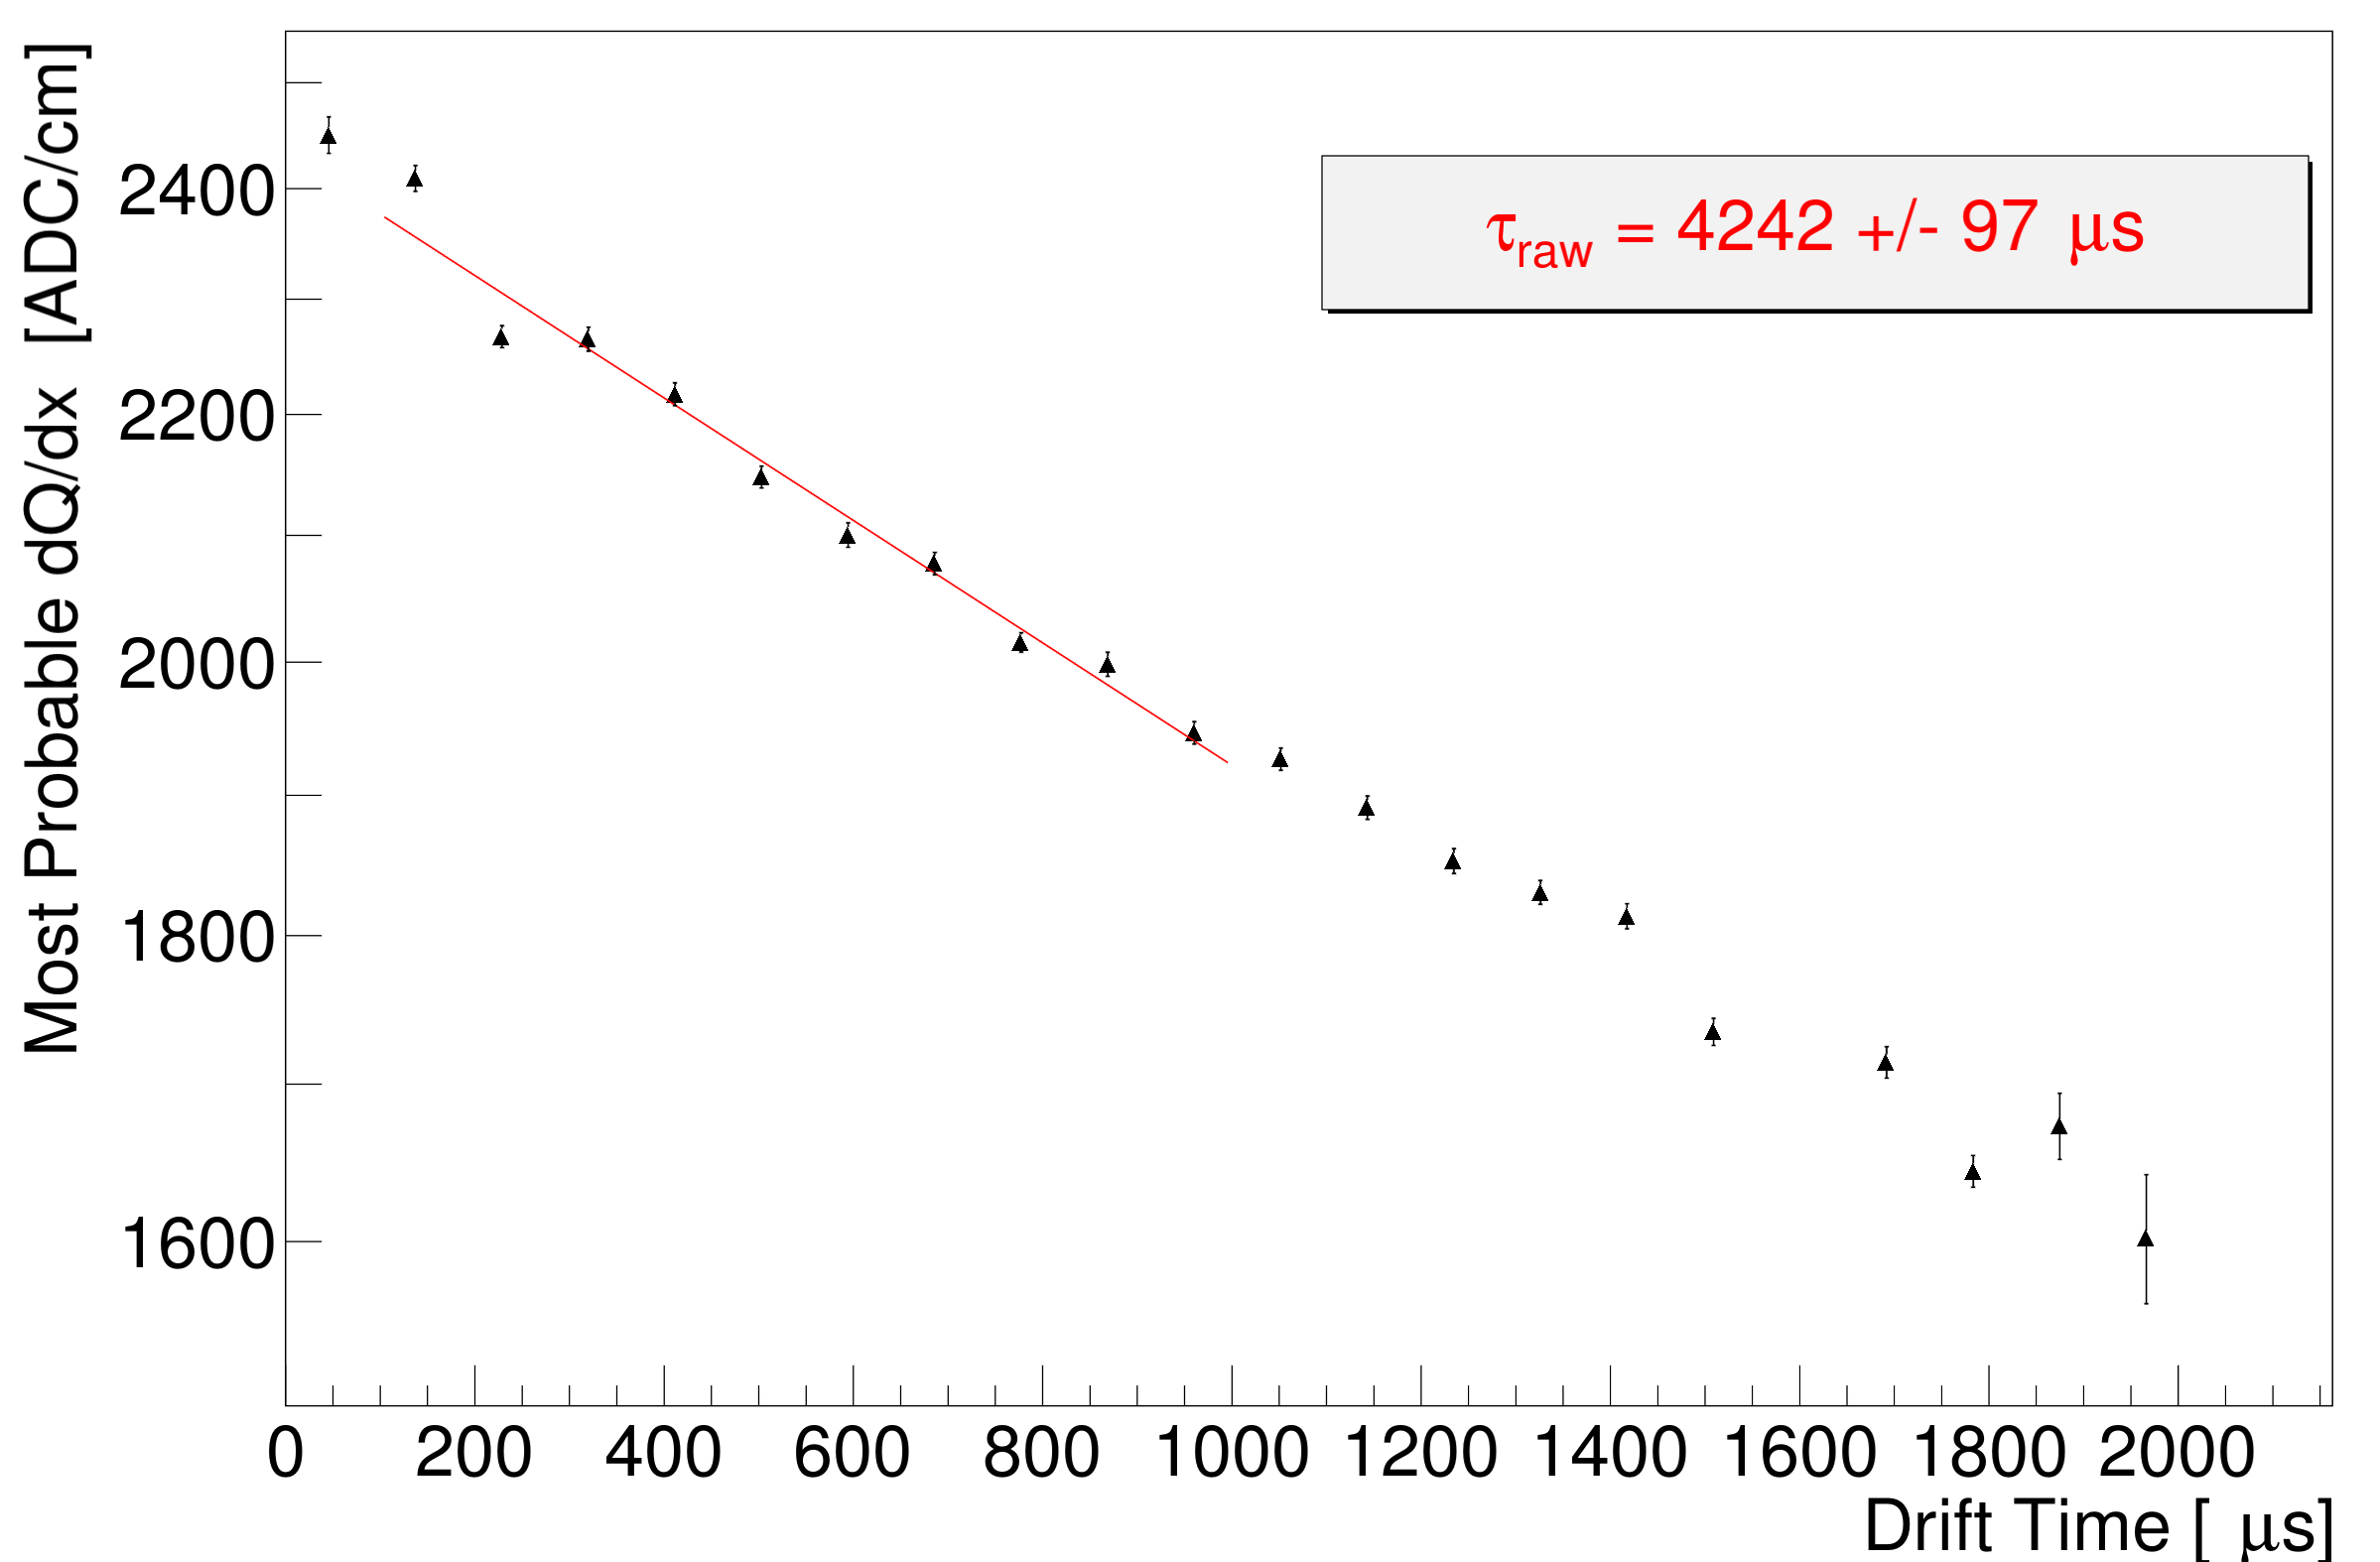
\includegraphics[width=0.7\textwidth]{canvMPV.png}
\caption{Most probable hit $dQ/dx$ measured at the anode, as a function of drift time. Exponential fit to fiducial range shown in red.}
\label{fig:landMPV}
\end{figure}

\subsection{Examining the bias through simulations}\label{sec:lifetimebias}

The signal-to-noise ratio (S/N) and particular electronic noise characteristics of the 35-ton are hypothesized to be the most significant factors influencing the bias in the electron lifetime measurement. Phenomena such as the varying noise frequency spectrum across the whole data-taking run, the varying noise amplitudes across the run as well as across channels, and the coherent noise between channels with the same voltage regulator are not included in the standard Monte Carlo simulation of the detector. Therefore, to accurately reflect the 35-ton noise characteristics, a data-driven noise model was devised for the simulation which uses real 35-ton data waveforms to define the noise.

\subsubsection{Data-Driven Noise Simulation}\label{sec:datadrivennoise}

The simulation uses CRY~\cite{CRY} to generate a single muon per event in the 35-ton geometry using the provided muon direction and energy flux parameterisations. Events where the muon passes through an East-West counter trigger pair are kept and propagated through the Geant4 step in the normal LArSoft simulation~\cite{larsoft}. The detector simulation of the event proceeds without addition of the simulated electronic noise and the noiseless simulated wire signals are passed to the separate noise addition step.

The noise addition process combines the simulated noiseless waveforms with representative data noise waveforms. The data noise waveforms are taken from real 35-ton data events, from the same dataset as described in section~\ref{sec:lifetime}. To remove the impact of triggered particle signals in the data waveforms, smaller unbiased sub-slices of the data waveforms are used: the final 5200 ticks of each 15000 tick waveform (see section~\ref{sec:daq}) are guaranteed to be free of triggered particle signals as the negative ionization charge will have already drifted to the anode. Remaining untriggered particle signals in the data waveforms are kept as representative real backgrounds. Furthermore, data on channels that are missing or dead in the real data are discarded, accurately reflecting the varying run characteristics of the 35-ton detector.

The two source waveforms are combined by a scaled ADC-by-ADC addition. In order to simulate the effects of different possible levels of S/N, the simulated signal waveforms are scaled by a factor, $\mu$, which represents a relative multiplier on the true S/N of 35-ton data. For example, $\mu$=2.0 represents twice the S/N of the 35-ton data, or in other words, twice as much signal. Following the data-driven noise simulation, the BHF and THB are used to reconstruct hits and tracks and the electron lifetime analysis proceeds using exactly the same procedure as for real 35-ton data.

There were 80 simulated samples created using the process described here, each with the same initial $\sim$35,000 East-West triggered simulated cosmic muon events. Five electron lifetimes are simulated ($\tau_{\text{MC}}=2.5,3.0,3.5,4.0,4.5$~ms), and for each lifetime, 16 different $\mu$ factors are simulated, ranging from 0.5 to 2.0 in increments of 0.1.

\subsubsection{Hit Reconstruction Purity and Efficiency}\label{sec:hitefficiency}

The performance of the BHF and THB on real and simulated data is summarised by the efficiency and purity statistics. In each simulated event, the reconstructed hit times are compared with the Monte Carlo truth information from the simulation to determine which reconstructed hits are ``true''. Reconstructed hits are ``true'' if there is at least one MC truth charge deposit on the same channel within $\pm 150$ ticks of the reconstructed hit peak time. Efficiency, $\epsilon_S$, is then defined as the number of reconstructed hits with matching MC truth hits divided by the total number of MC truth hits. Purity, $\phi$, is defined as the number of MC-matched reconstructed hits divided by the total number of reconstructed hits. For the simulations, the hit finding efficiency and purity are calculated as functions of drift distance, as in figure~\ref{fig:pureff}, and as functions of $\mu$, as in figure~\ref{fig:pureffvnoise}. The purity of reconstruction is high ($>94\%$) for all simulated samples, even if the simulated noise is higher than the 35-ton noise. Thus, it can be said that if a hit is found, then it is highly likely to be a real hit, a direct consequence of the robust MLESAC algorithm implementation described in section~\ref{sec:hitfinder}. Similarly, the efficiency is high for hits near the anode and in the presence of low detector noise, but drops to around 75\% for longer drifts and higher noise. At long drift lengths, the drifting charge is partially absorbed by impurities and the signal is often below the hit finding threshold, thereby reducing the efficiency despite the assumption of hit locations based on neighboring large charge hits in the BHF. 

The dependence of efficiency on drift distance is a motive to apply a fiducial cut on the sensitive region of the TPC, nearer to the APA. The steep drop in efficiency for detectors with higher noise than the 35-ton (lower $\mu$) reinforces the necessity for low-noise readout in order to efficiently and accurately reconstruct events. 

\begin{figure}
\centering
\begin{subfigure}{0.45\textwidth}
\centering
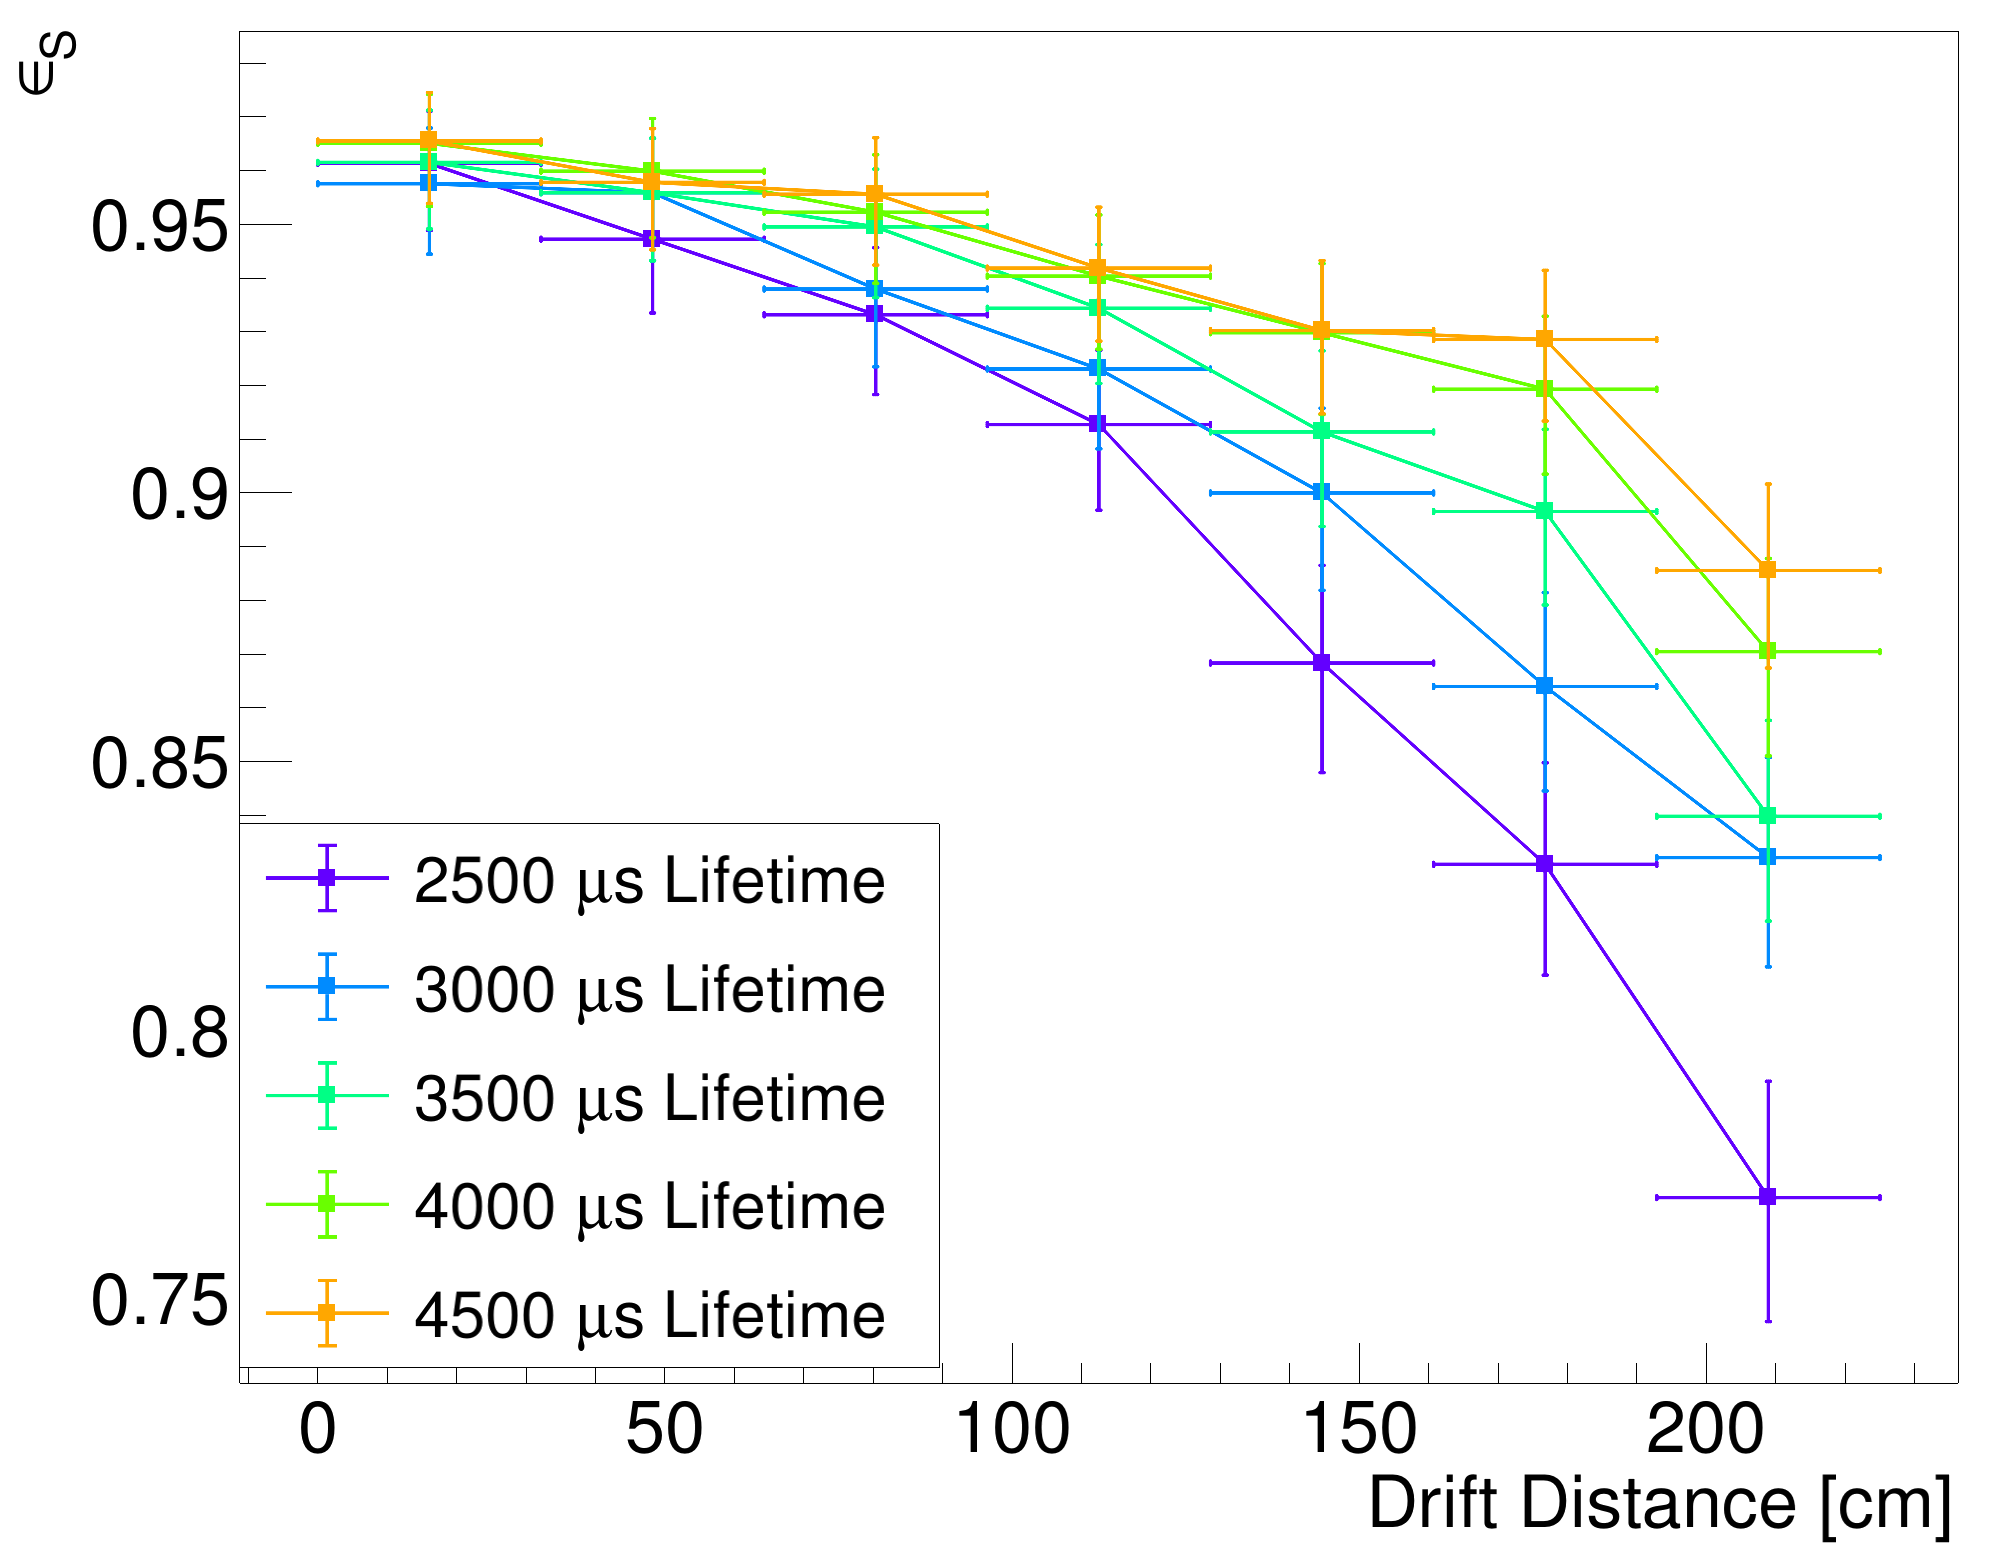
\includegraphics[width=\textwidth]{canveffdriftlife.png}
\end{subfigure}
\begin{subfigure}{0.45\textwidth}
\centering
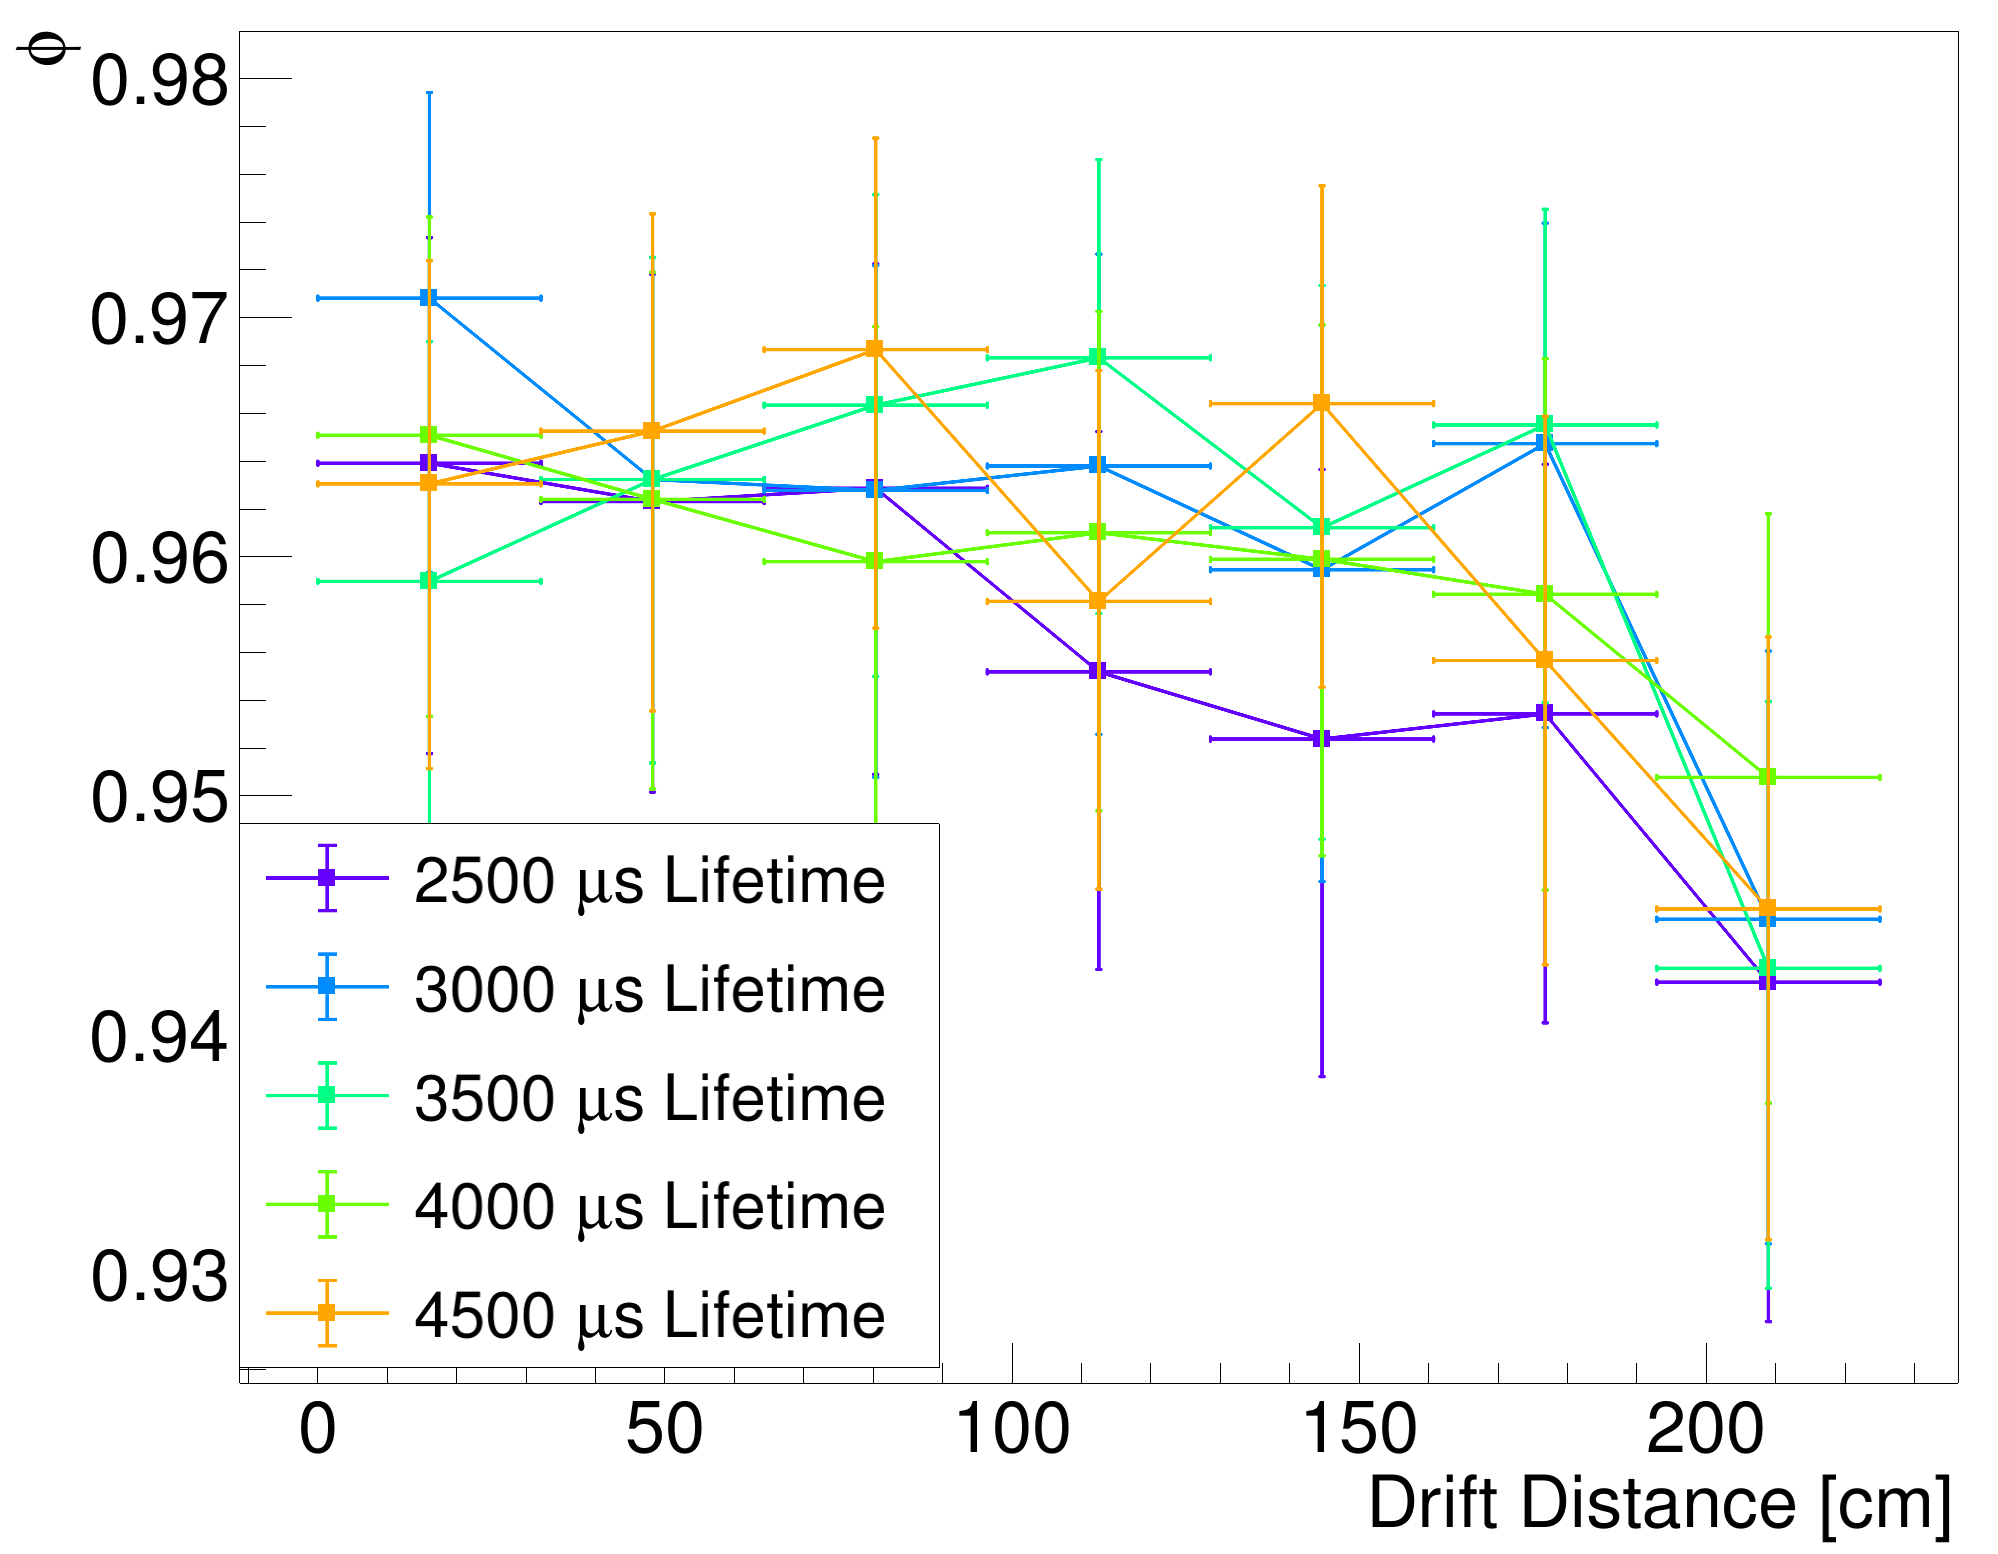
\includegraphics[width=\textwidth]{canvpurdriftlife.png}
\end{subfigure}
\caption{Efficiency (left) and purity (right) of hit finding in the simulation as functions of drift distance for $\mu=1.2$ and several values of $\tau_{\text{MC}}$.}
\label{fig:pureff}
\end{figure}

\begin{figure}
\centering
\begin{subfigure}{0.45\textwidth}
\centering
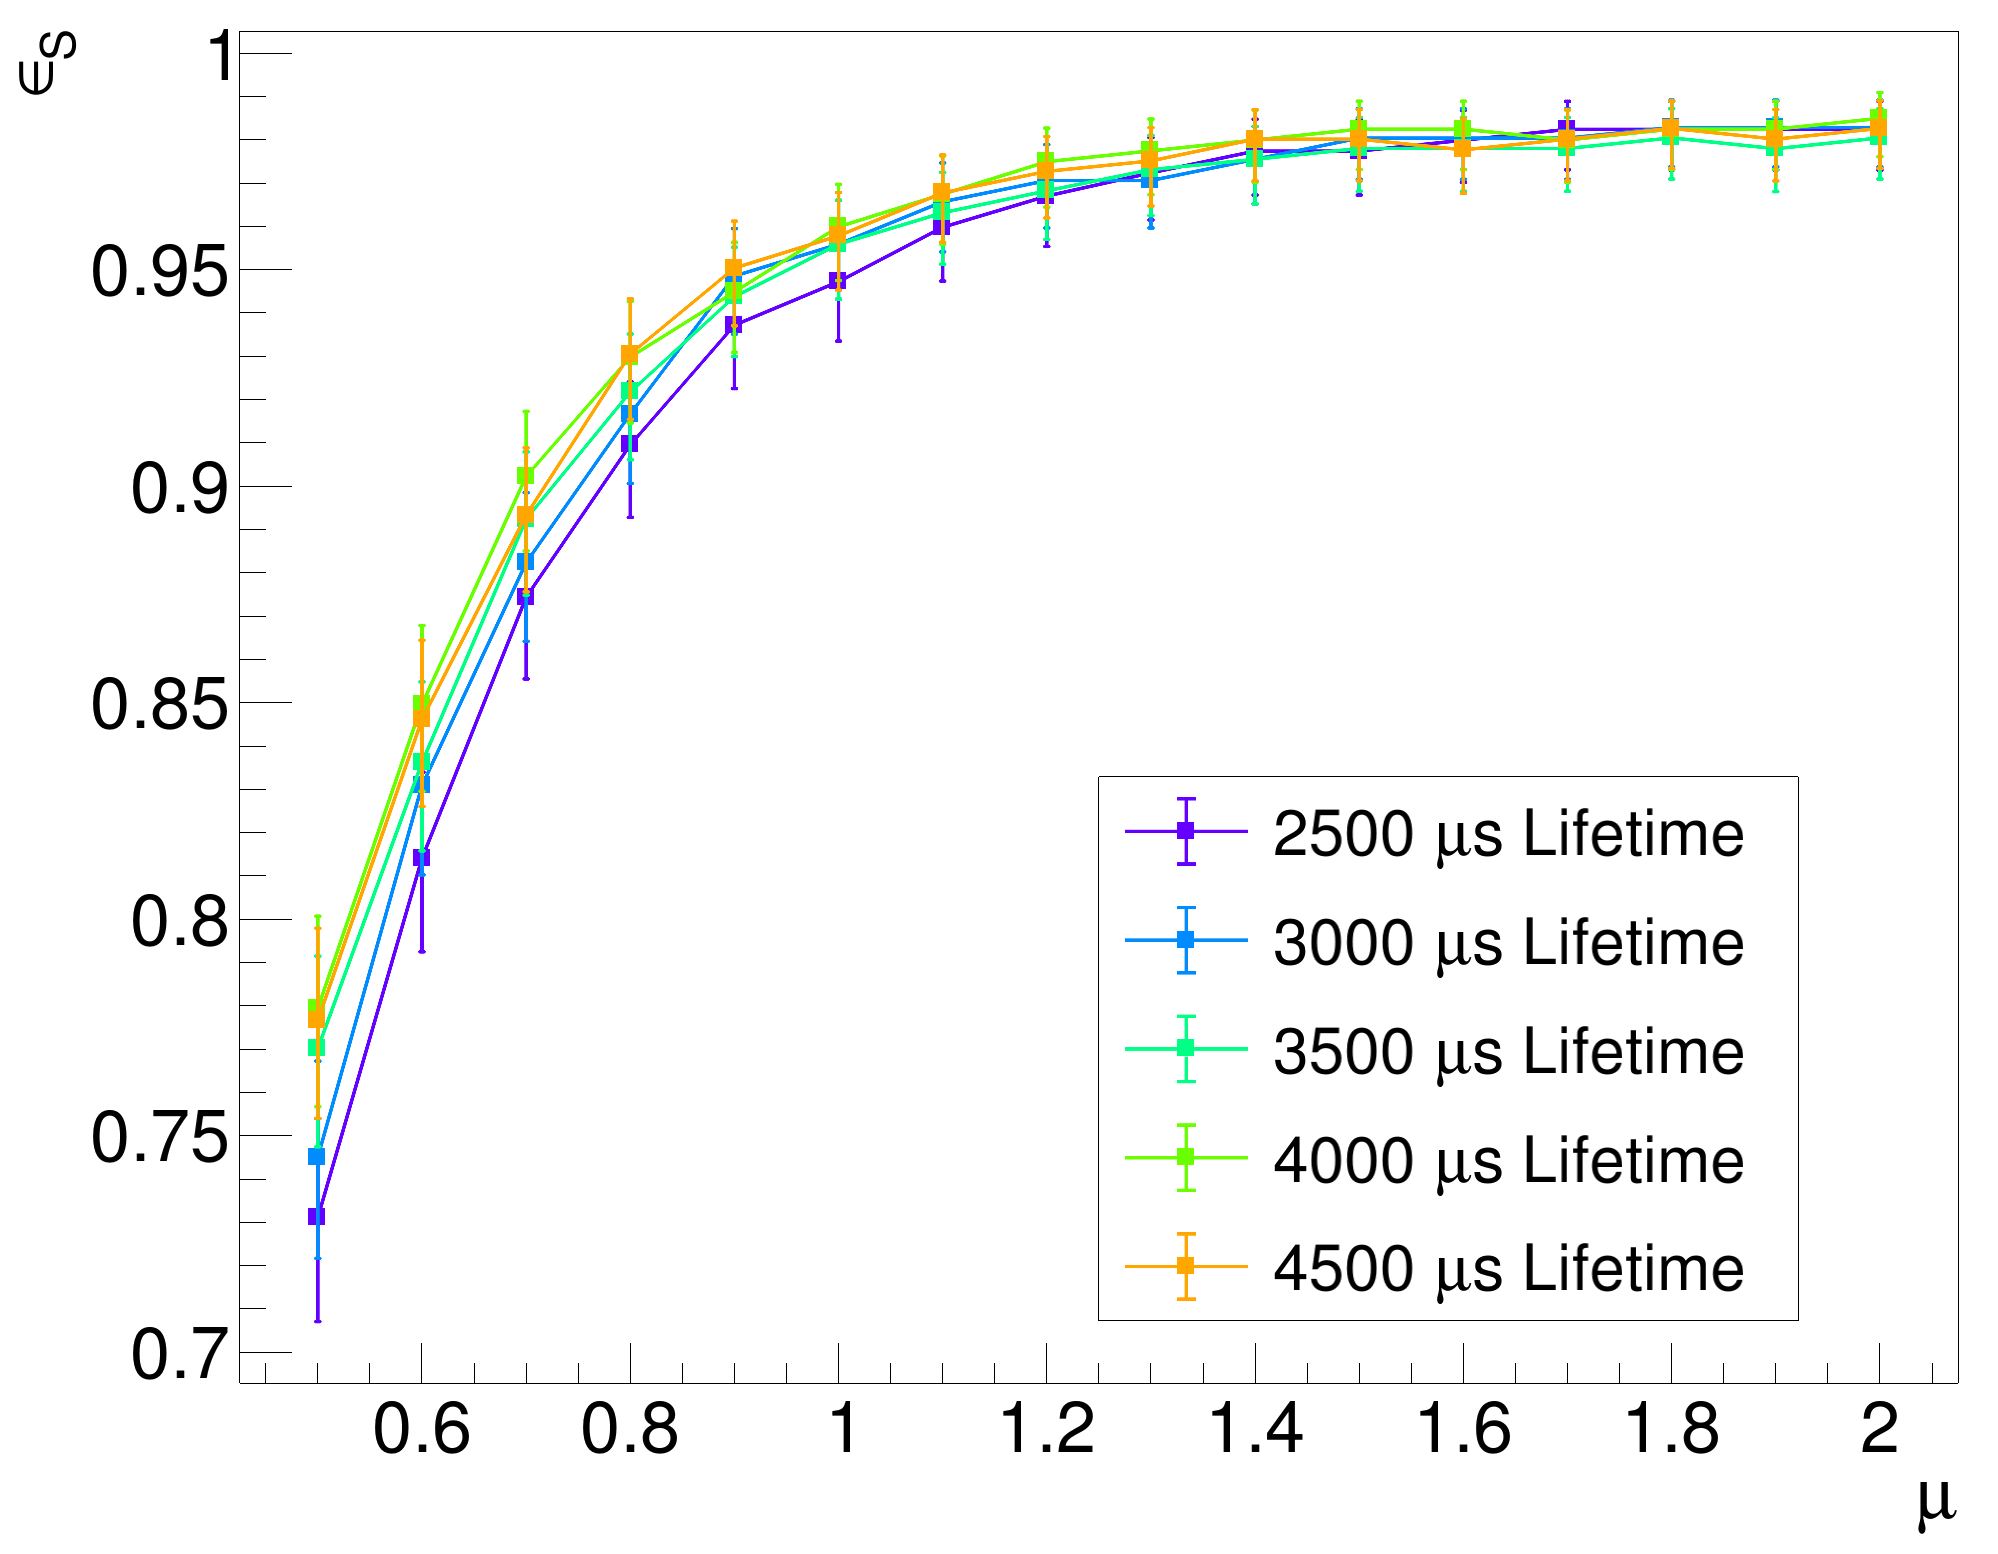
\includegraphics[width=\textwidth]{effvnoise.png}
\end{subfigure}
\begin{subfigure}{0.45\textwidth}
\centering
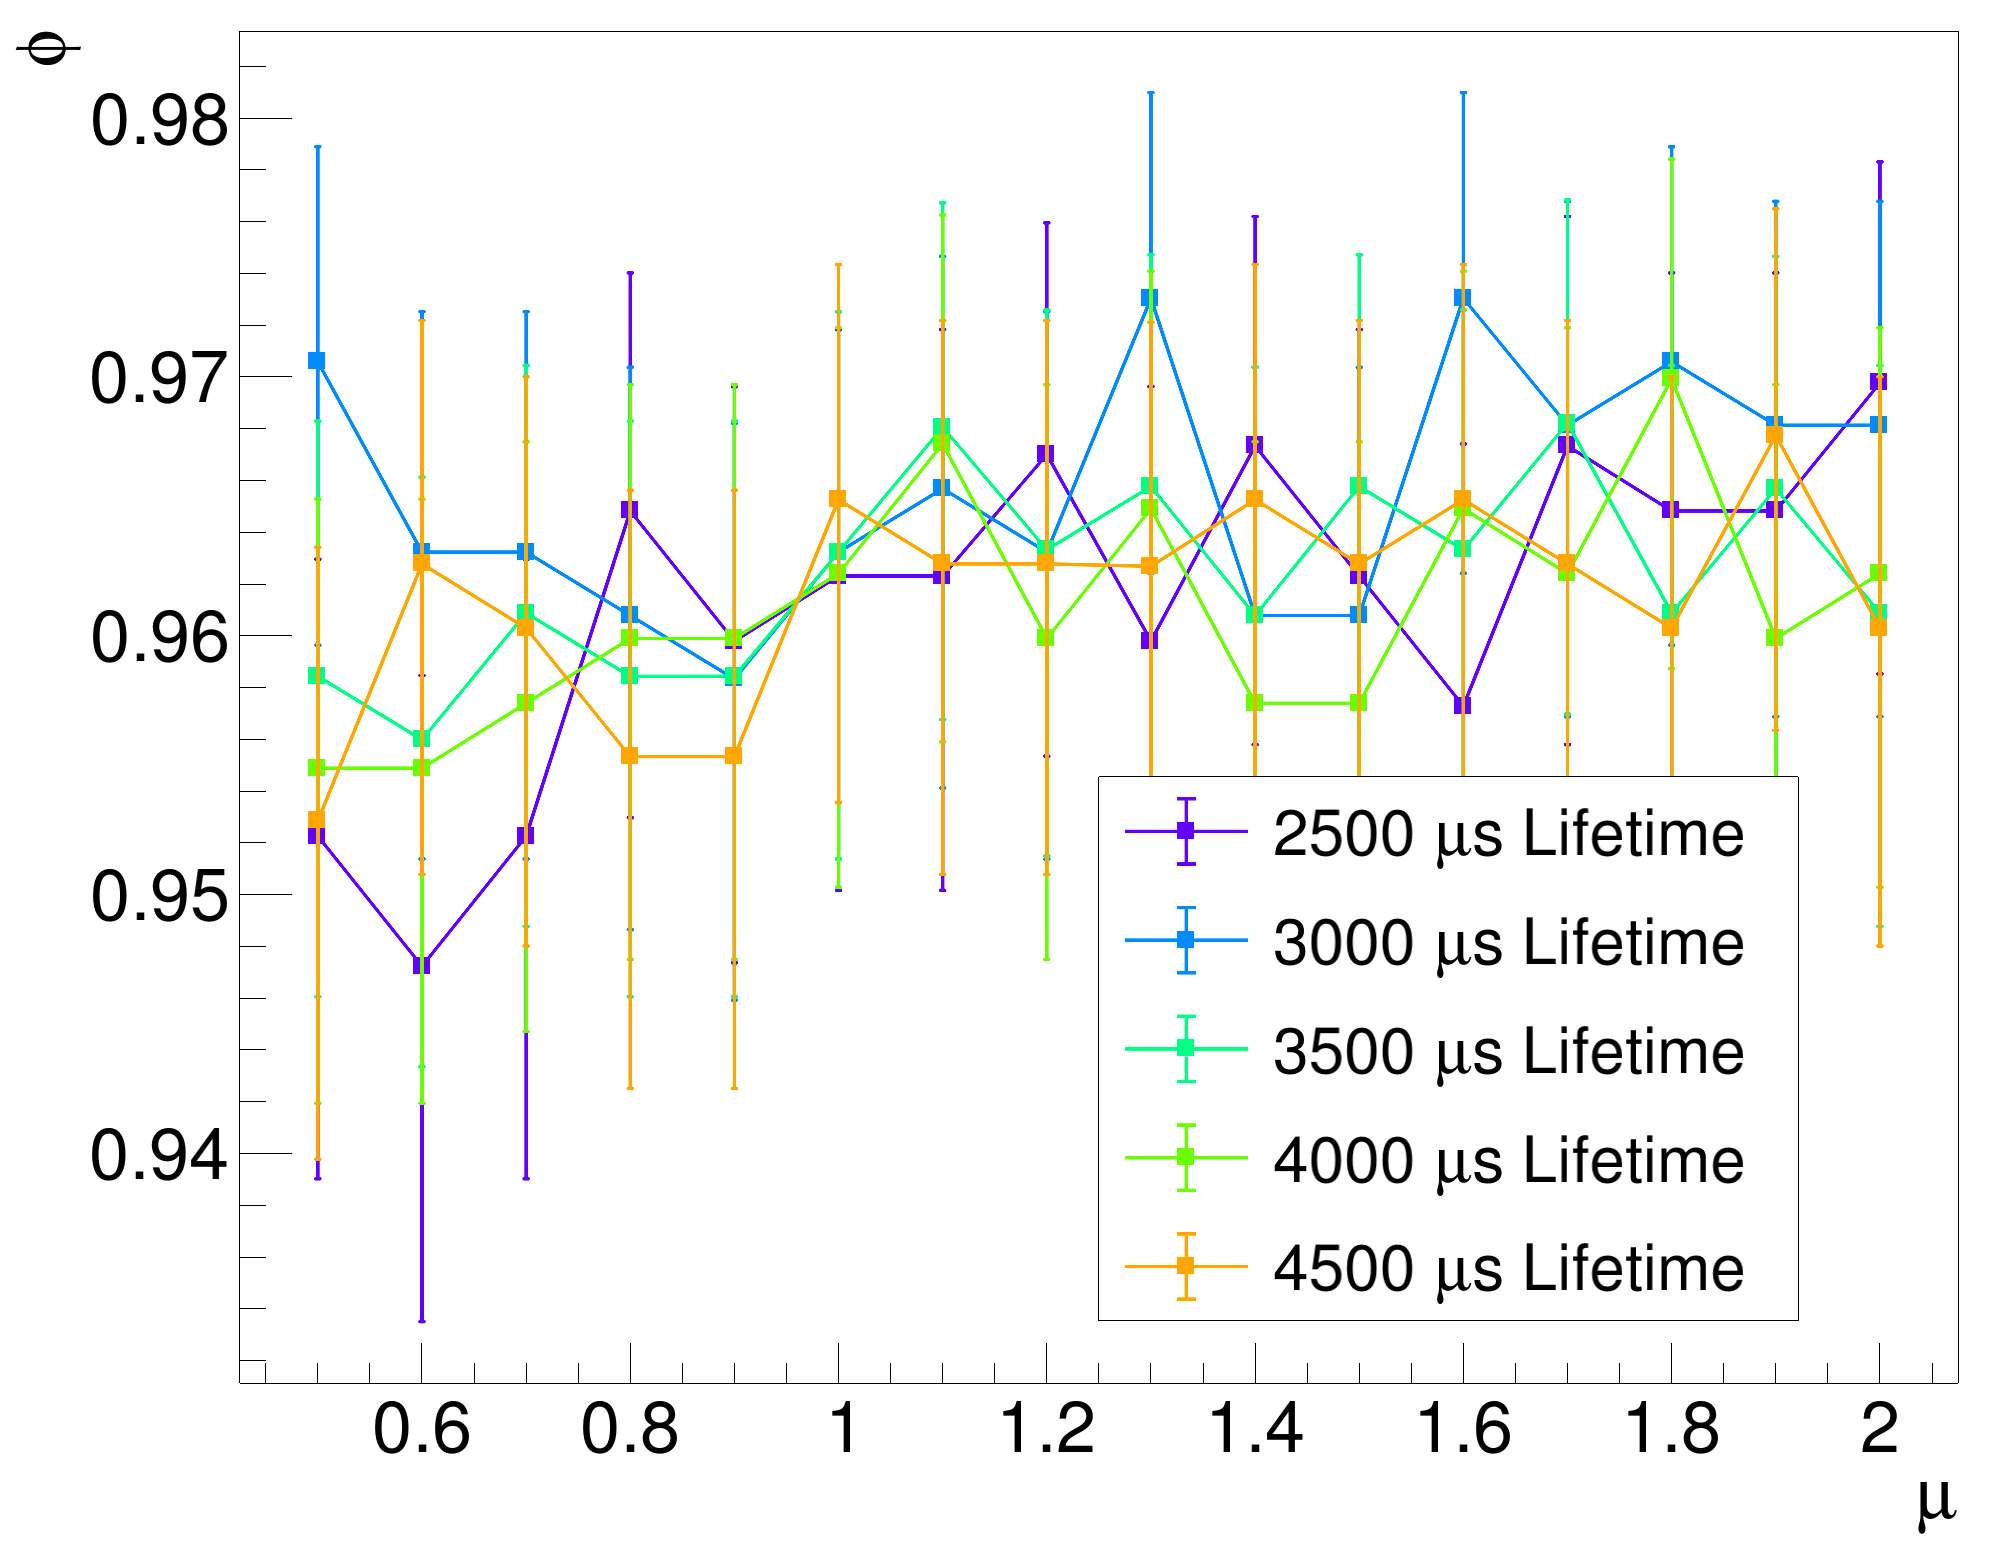
\includegraphics[width=\textwidth]{purvnoise.png}
\end{subfigure}
\caption{Efficiency (left) and purity (right) of hit finding as functions of $\mu$ for muon counter triggers 9 and 31 ($44\pm15$~cm drift distance) and several values of $\tau_{\text{MC}}$.}
\label{fig:pureffvnoise}
\end{figure}

\subsubsection{Hit Efficiency and Charge Resolution}\label{sec:chgresolution}

The hit efficiency and charge resolution of the BHF, with respect to true MC charge, together illustrate the main source of bias in this analysis. Figure~\ref{fig:effcharge} shows the hit finding efficiency with respect to simulated hit charge, as well as the simulated hit charge distribution. The sigmoid efficiency function cuts off a portion of the charge distribution so smaller charge hits are less likely to be reconstructed than larger charge hits, therefore causing a bias in the true Landau MPV determination. Further, as the Landau MPV shifts down due to charge attenuation over drift, an increasing fraction of the distribution goes below the efficiency threshold, and causes the apparent MPV to level off around the sigmoid function cutoff, even though the true MPV continues to decrease. This then biases the observed lifetime, $\tau_{\text{raw}}$, toward higher values for longer drifts, away from the true lifetime. The impact of this effect alone is small, as the THB recovers low charge hits as long as they are interpolable from existing reconstructed hits.

Figure~\ref{fig:chgresol} shows the charge resolution, $\sigma_q$, defined as the FWHM of the standardised charge residual distribution, $\left(Q_{Reco}-Q_{MC}\right)/Q_{MC}$, as a function of hit charge. In the range of $Q_{MC}$ relevant to this analysis and for detector noise similar to the 35-ton data, $\sigma_q$ ranges from below 20\% to above 70\%. The varying resolution across this range implies a modified detector Gaussian resolution function where the width parameter is a function of hit charge. This alternative parameterisation of the Landau-Gaussian convolution fit function is not studied here, although it is assumed that these model-dependent differences contribute a large systematic uncertainty despite good fits across all drift bins ($0.9<\chi^2/\text{N.D.F.}<1.5$). The uncertainty arises as the true Landau MPV does not correspond to the value which is parameterised in the fit function. Therefore, to account for the effects of the varying charge resolution and low hit efficiency for small charge hits, a systematic uncertainty is associated with the magnitude of overall bias in the lifetime parameter (see section~\ref{sec:lifetimesystematics} for more discussion).

\begin{figure}
\centering
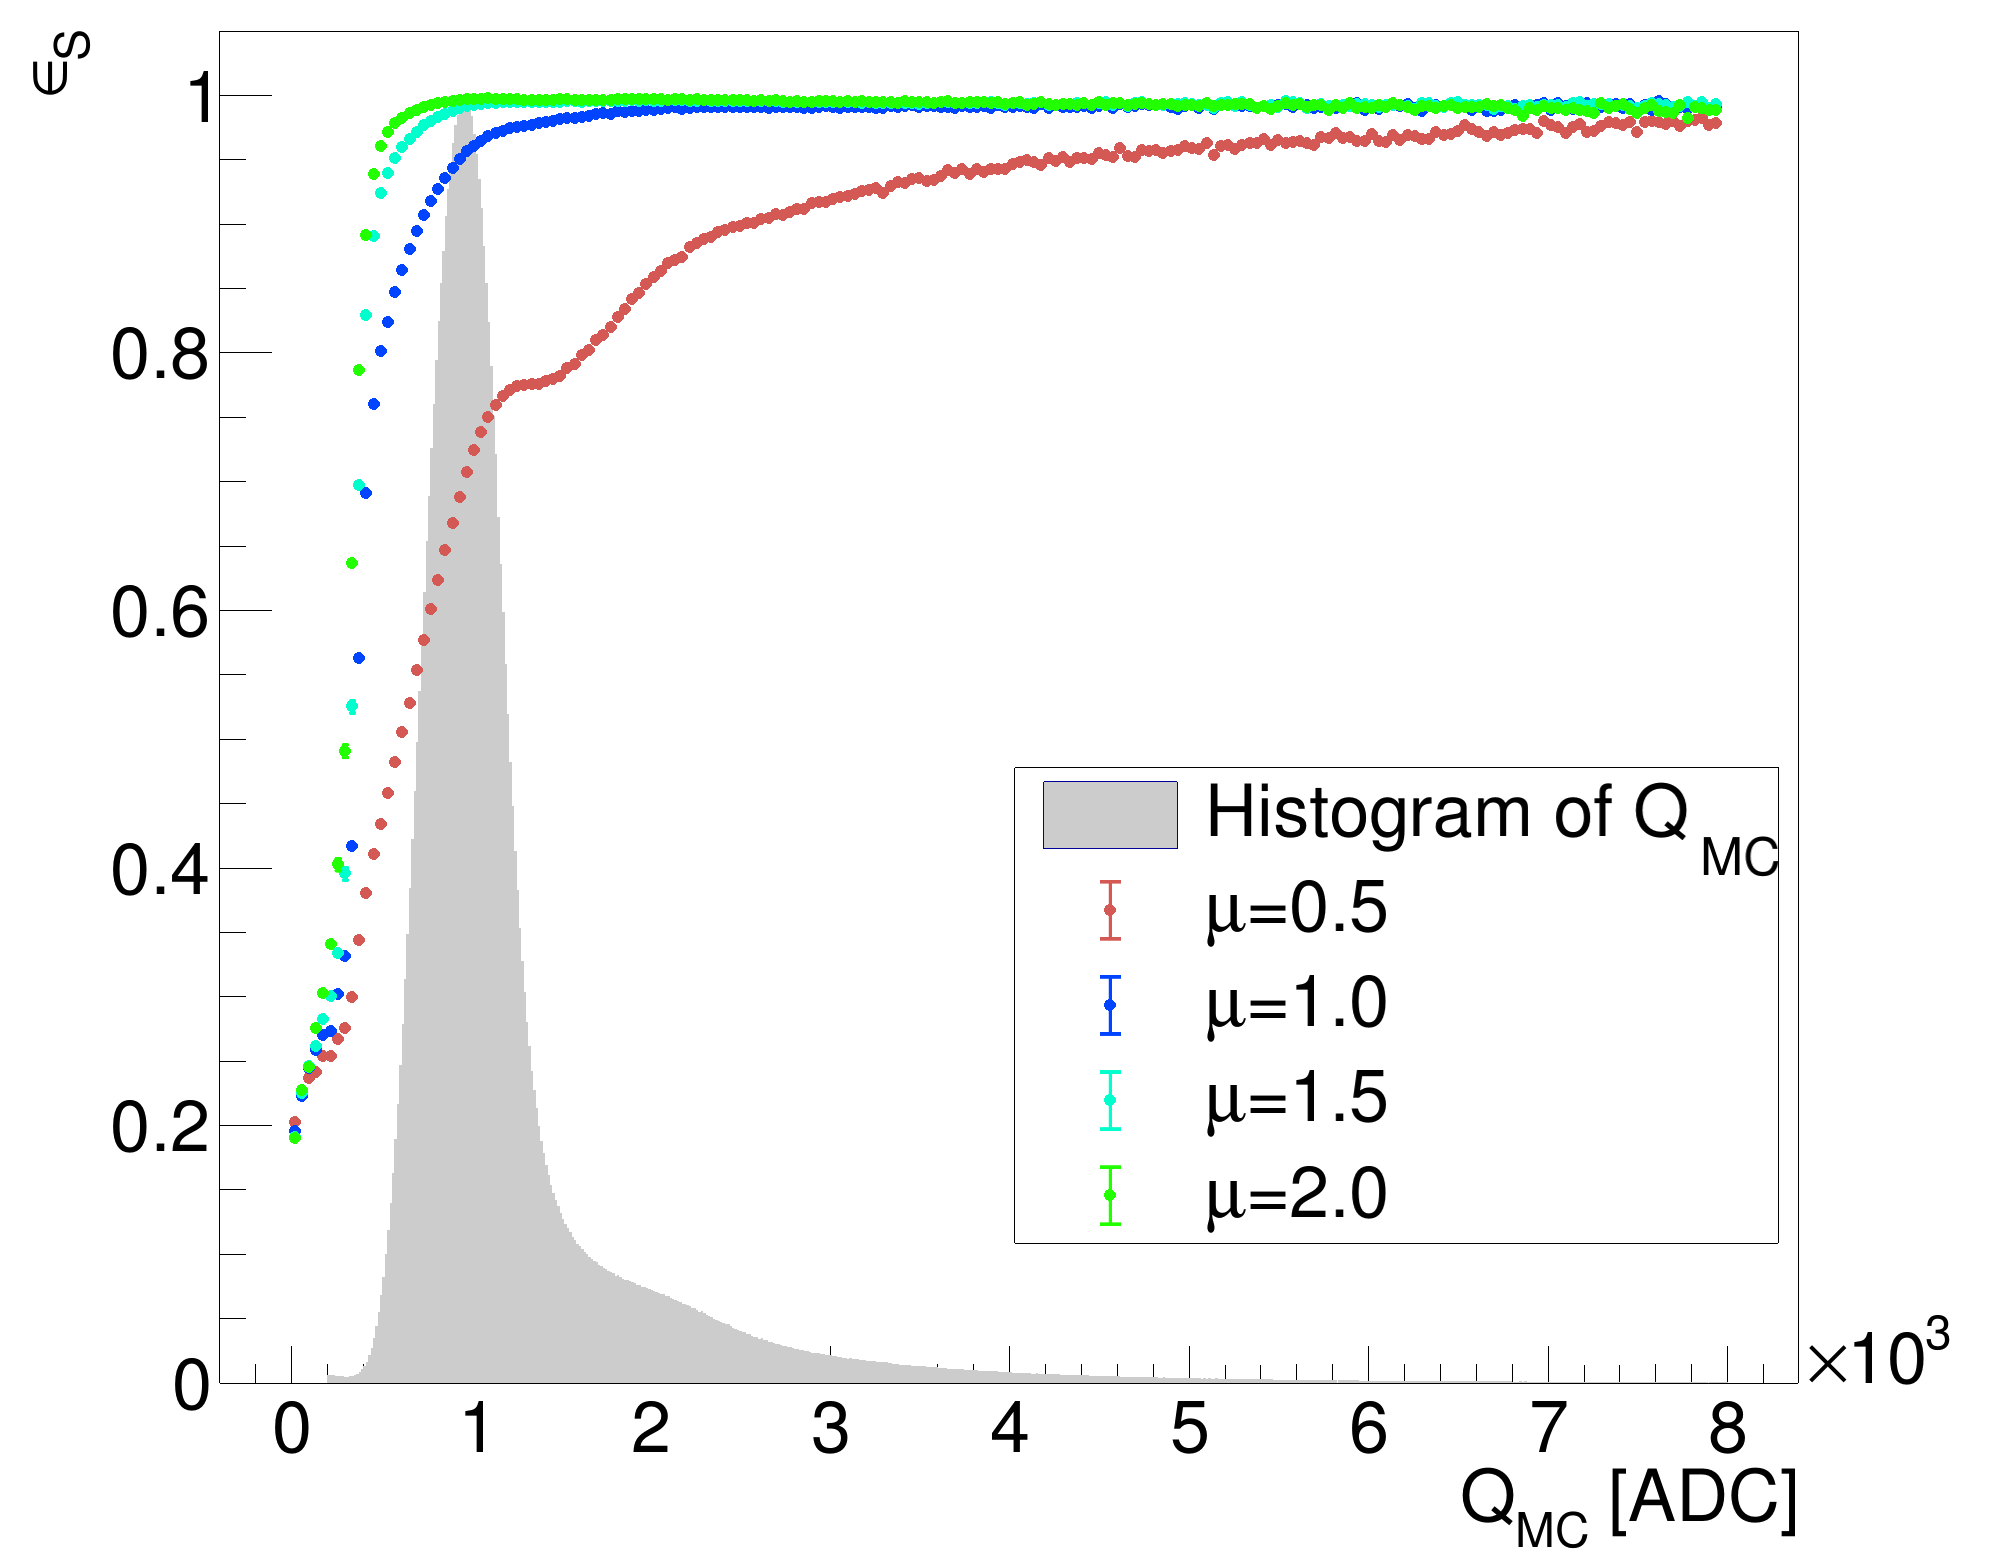
\includegraphics[width=0.6\textwidth]{effcharge.png}
\caption{Hit finding efficiency vs. hit charge for several values of $\mu$. The histogram (arbitrary normalization) of MC hit charge is shown in shaded gray for comparison.}
\label{fig:effcharge}
\end{figure}

\begin{figure}
\centering
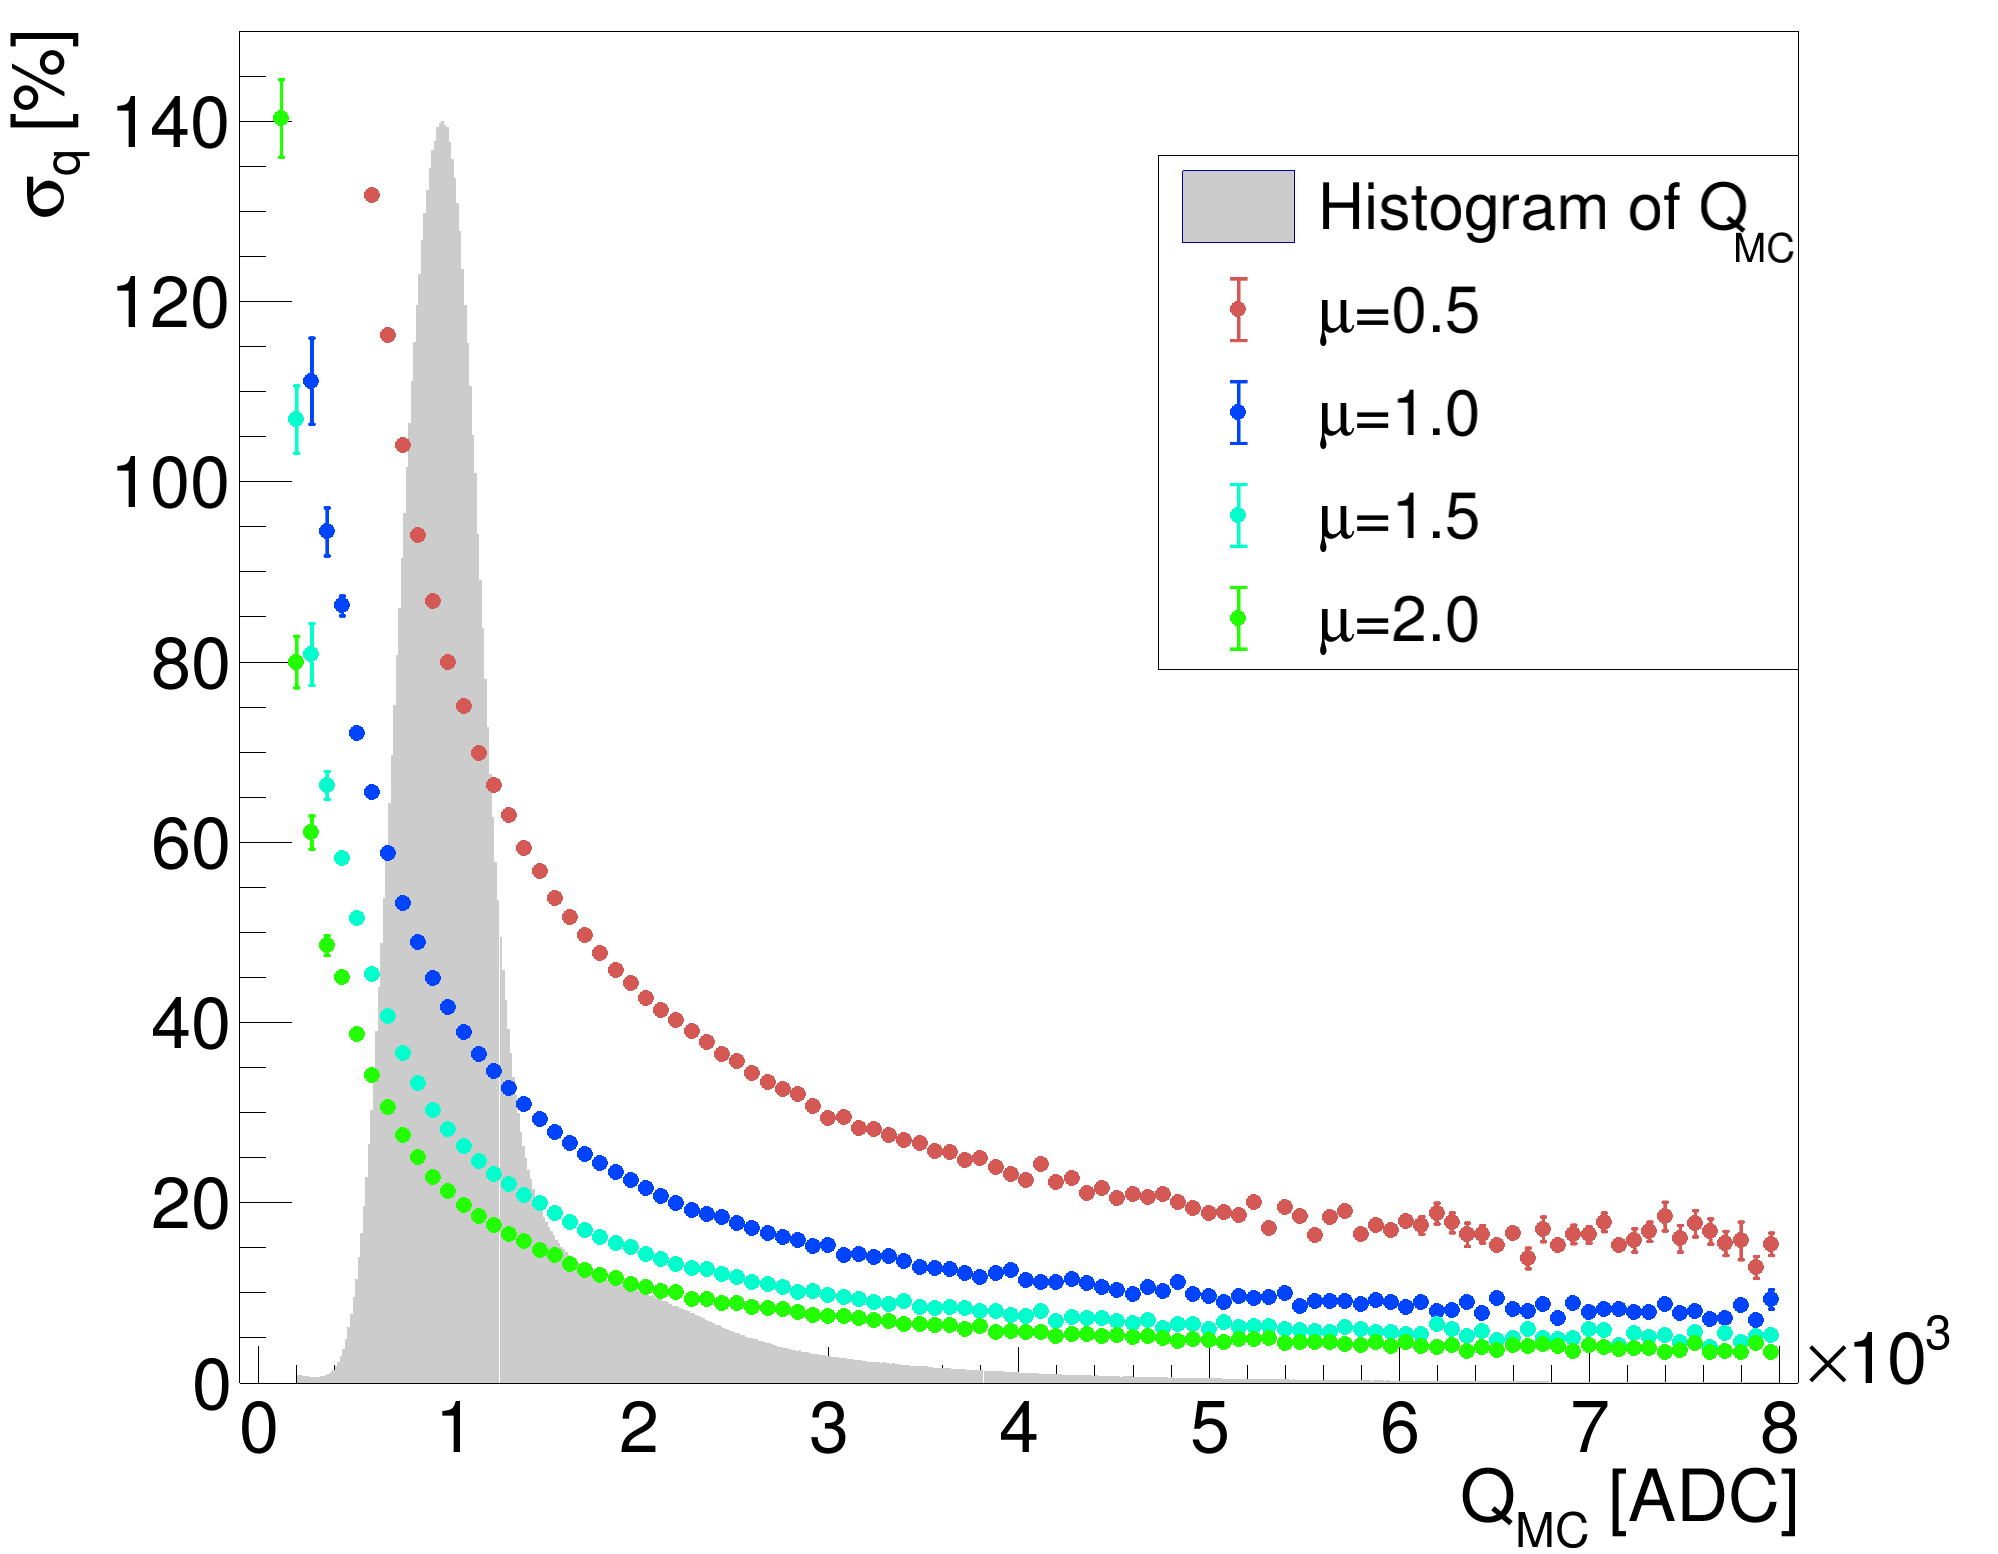
\includegraphics[width=0.6\textwidth]{resolution.png}
\caption{Charge resolution vs. hit charge for several values of $\mu$. The histogram (arbitrary normalization) of MC hit charge is shown in shaded gray for comparison.}
\label{fig:chgresol}
\end{figure}

\subsubsection{Fiducial Cut}\label{sec:fiducialcut}

A consequence of the poor charge resolution and hit efficiency for small charge hits is the increase in systematic uncertainty of the Landau MPV for bins of longer drift, and hence the bias in the lifetime, as described in section~\ref{sec:chgresolution}. This drift distance dependent phenomenon motivates a fiducial cut for the lifetime measurement. Defining a threshold for this cut, however, is not possible without prior knowledge of the true argon lifetime. Nevertheless, it is known that there is \emph{less} bias in the measured hit charges with shorter drift times (near the anode) than with longer drift times (near the cathode). Additionally, the first drift time bin is ignored from the lifetime measurement to reduce the influence of charge deposits within the wire planes, which are not yet well-modelled. Based on these observations, an arbitrary fiducial cut of 5-50\% the full drift time is imposed to reduce the bias and the systematic uncertainty on the electron lifetime measurement. Stricter cuts on drift time are hypothesized to reduce the bias and uncertainty even further, but these dependencies are not studied. To illustrate the effectiveness of the 5-50\% cut on the lifetime bias, $\tau_{\text{raw}}$ from the full detector drift distance is observed as $4.73$~ms, compared with $4.24$~ms with the cut imposed (see figure~\ref{fig:landMPV}). A drift distance dependent upward bias on $\tau_{\text{raw}}$ clearly exists, and is attributed to the decreasing hit efficiency and worsening charge resolution at longer drift lengths. Quantifying the bias and systematic uncertainty on the observed lifetime is done by comparing the lifetimes measured from the simulated samples to the true simulated lifetime.

\subsubsection{Signal Simulation Scaling}\label{sec:chanscale}

While all aspects of the 35-ton electronic noise are directly reproduced in the simulation, uncertainty remains in the collection wire signal simulation. The most probable charge deposited in the TPC in the absence of charge attenuation due to impurities is given by the intercept parameter in the exponential fit (equation~\ref{eq:lifetime}), $(dQ/dx)_0$. Comparison of 35-ton data, $(dQ/dx)_0$=2433~ADC/cm, and the simulated sample with $\mu$=1.0, $(dQ/dx)_0$=2099~ADC/cm, shows that the simulation does not accurately model the true S/N of 35-ton data (figure~\ref{fig:dqdx0scale}). Instead, scaling up the amplitude of signal simulation by an additional 15.3\% more closely resembles the 35-ton data, though further study of the causes of these differences is not pursued. The remaining differences between simulation and 35-ton data are included in the overall estimation of systematic uncertainty.

\begin{figure}
\centering
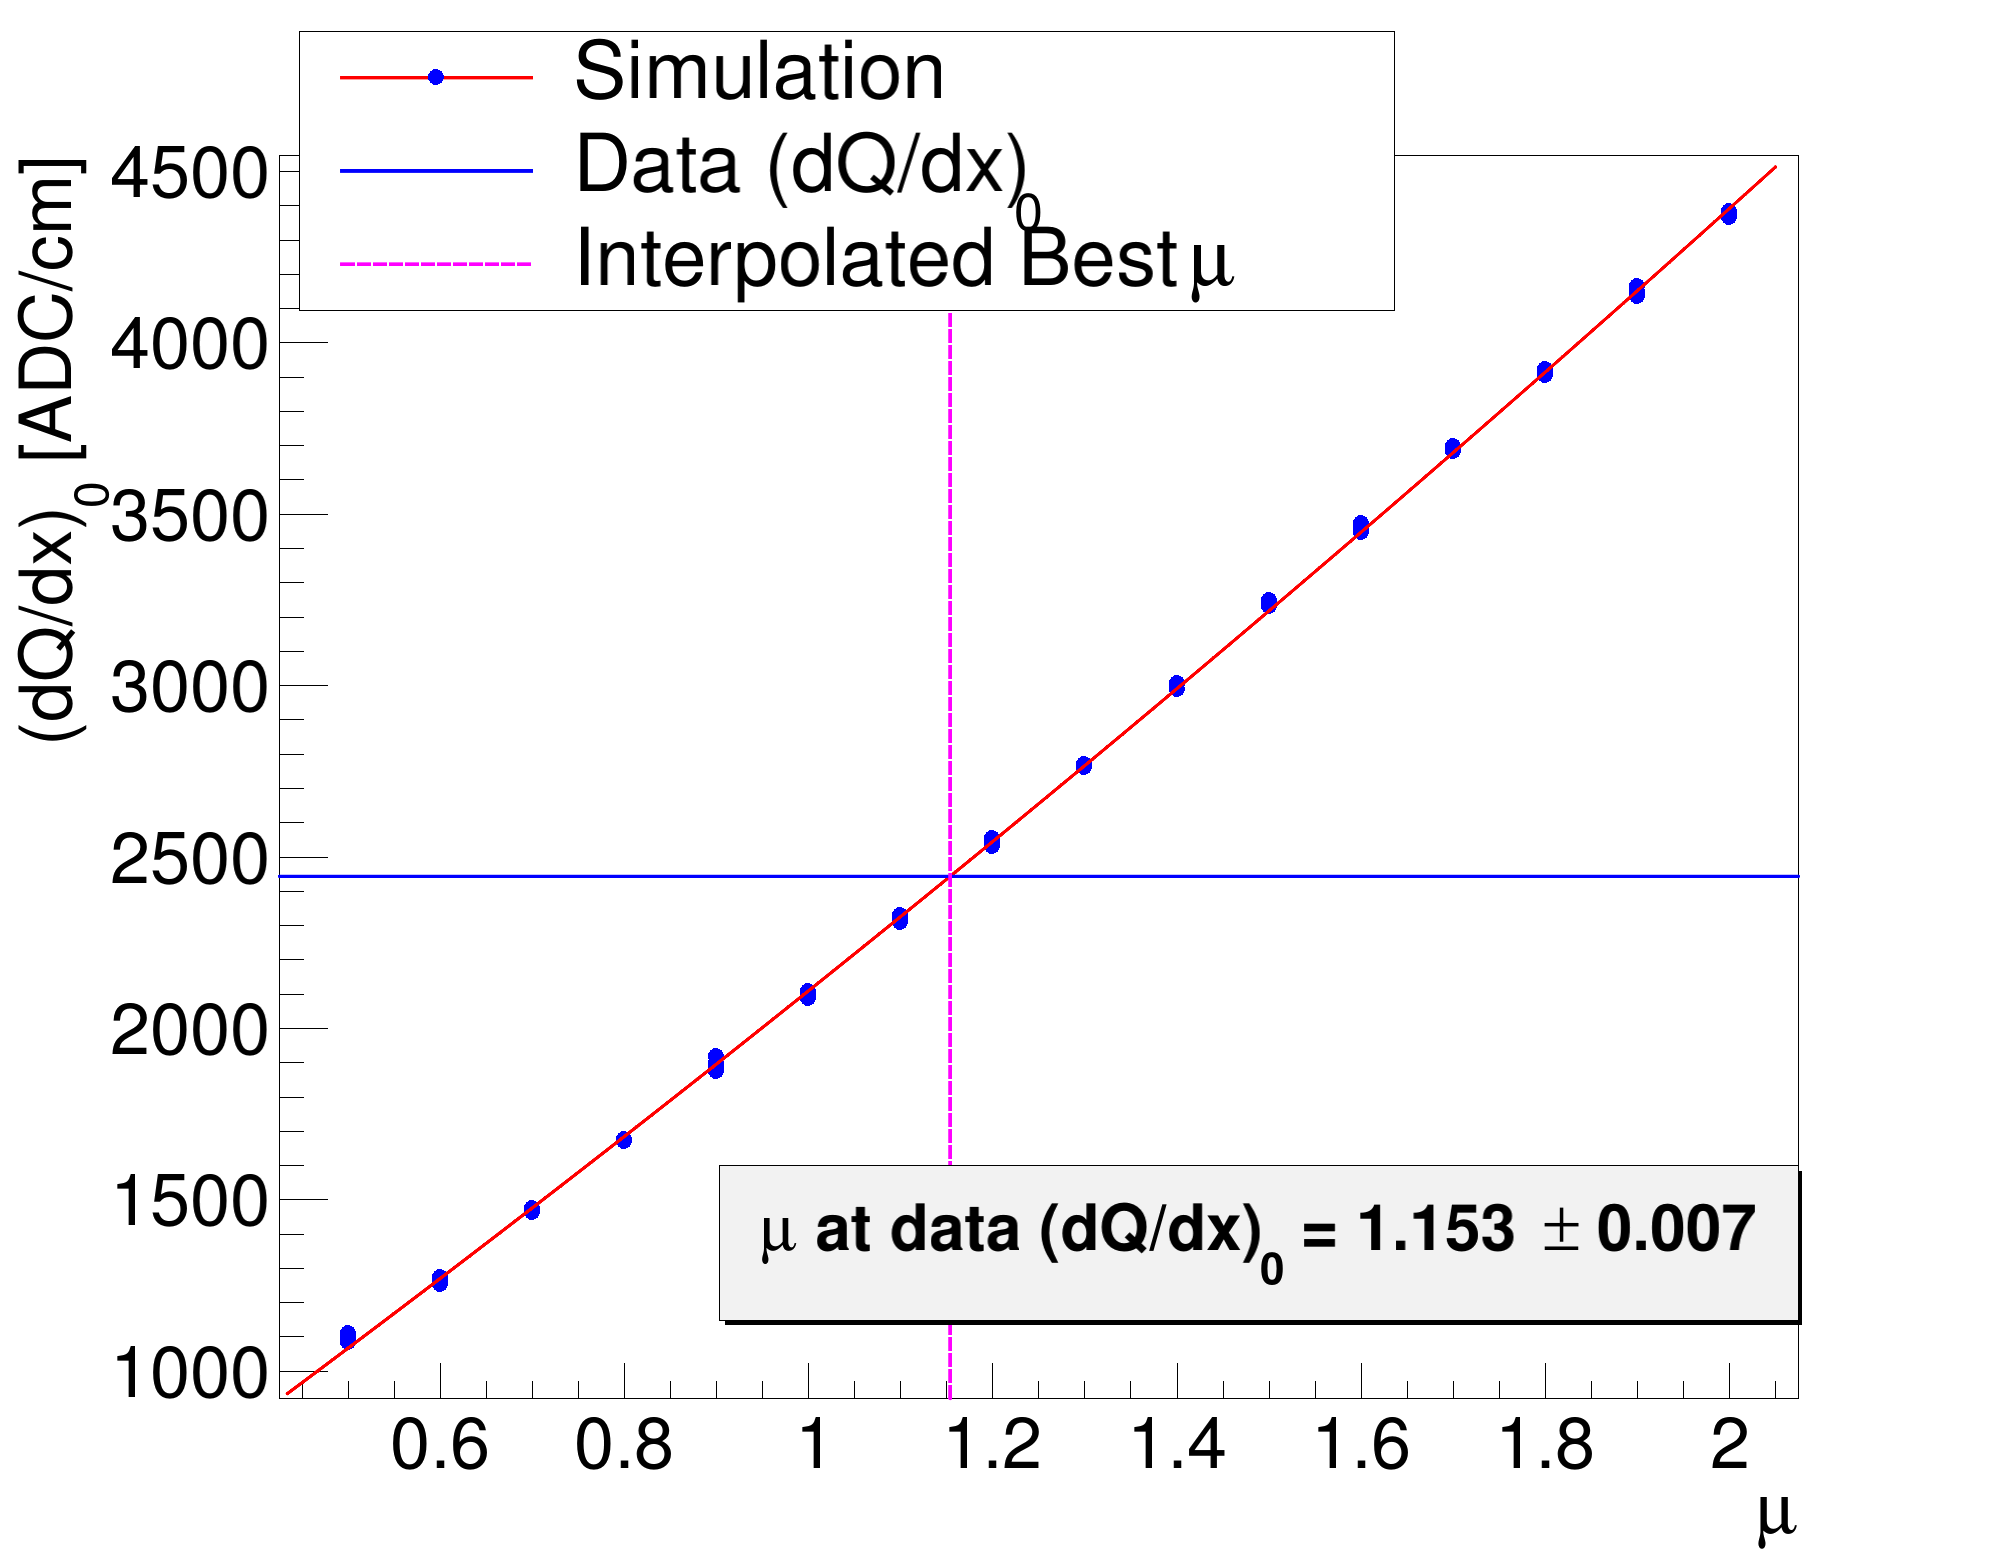
\includegraphics[width=0.6\textwidth]{canvdqdx0.png}
\caption{Exponential fit intercept $(dQ/dx)_0$ parameter for all simulated samples.}
\label{fig:dqdx0scale} 
\end{figure}

\subsection{Correcting for Lifetime Bias}\label{sec:debiasing}

By analyzing the electron lifetime of many simulated samples of varying parameters and comparing the results with the measured data, the lifetime of the 35-ton dataset can be extracted. Figure~\ref{fig:elifeVnoise} shows the the observed raw lifetimes, as a function of noise level, separated by true simulated lifetime. For simulated samples, the horizontal scale is $\mu$/1.153, correcting for signal simulation error, as described in the previous section. The bias in the observed lifetime for higher noise can be seen for lower $\mu$ values, a result of the drift-dependent upward bias in Landau MPVs. The measured lifetime for the 35-ton data is consistent with the simulated samples with 4.0~ms lifetime, and $\mu$ of 1.1 and 1.2, confirmed by the similarities shown in figure~\ref{fig:mpvchoice}. The corrected electron lifetime of 35-ton data is more precisely determined through interpolation.

\begin{figure}
\centering
\begin{minipage}[t]{0.48\textwidth}
\centering
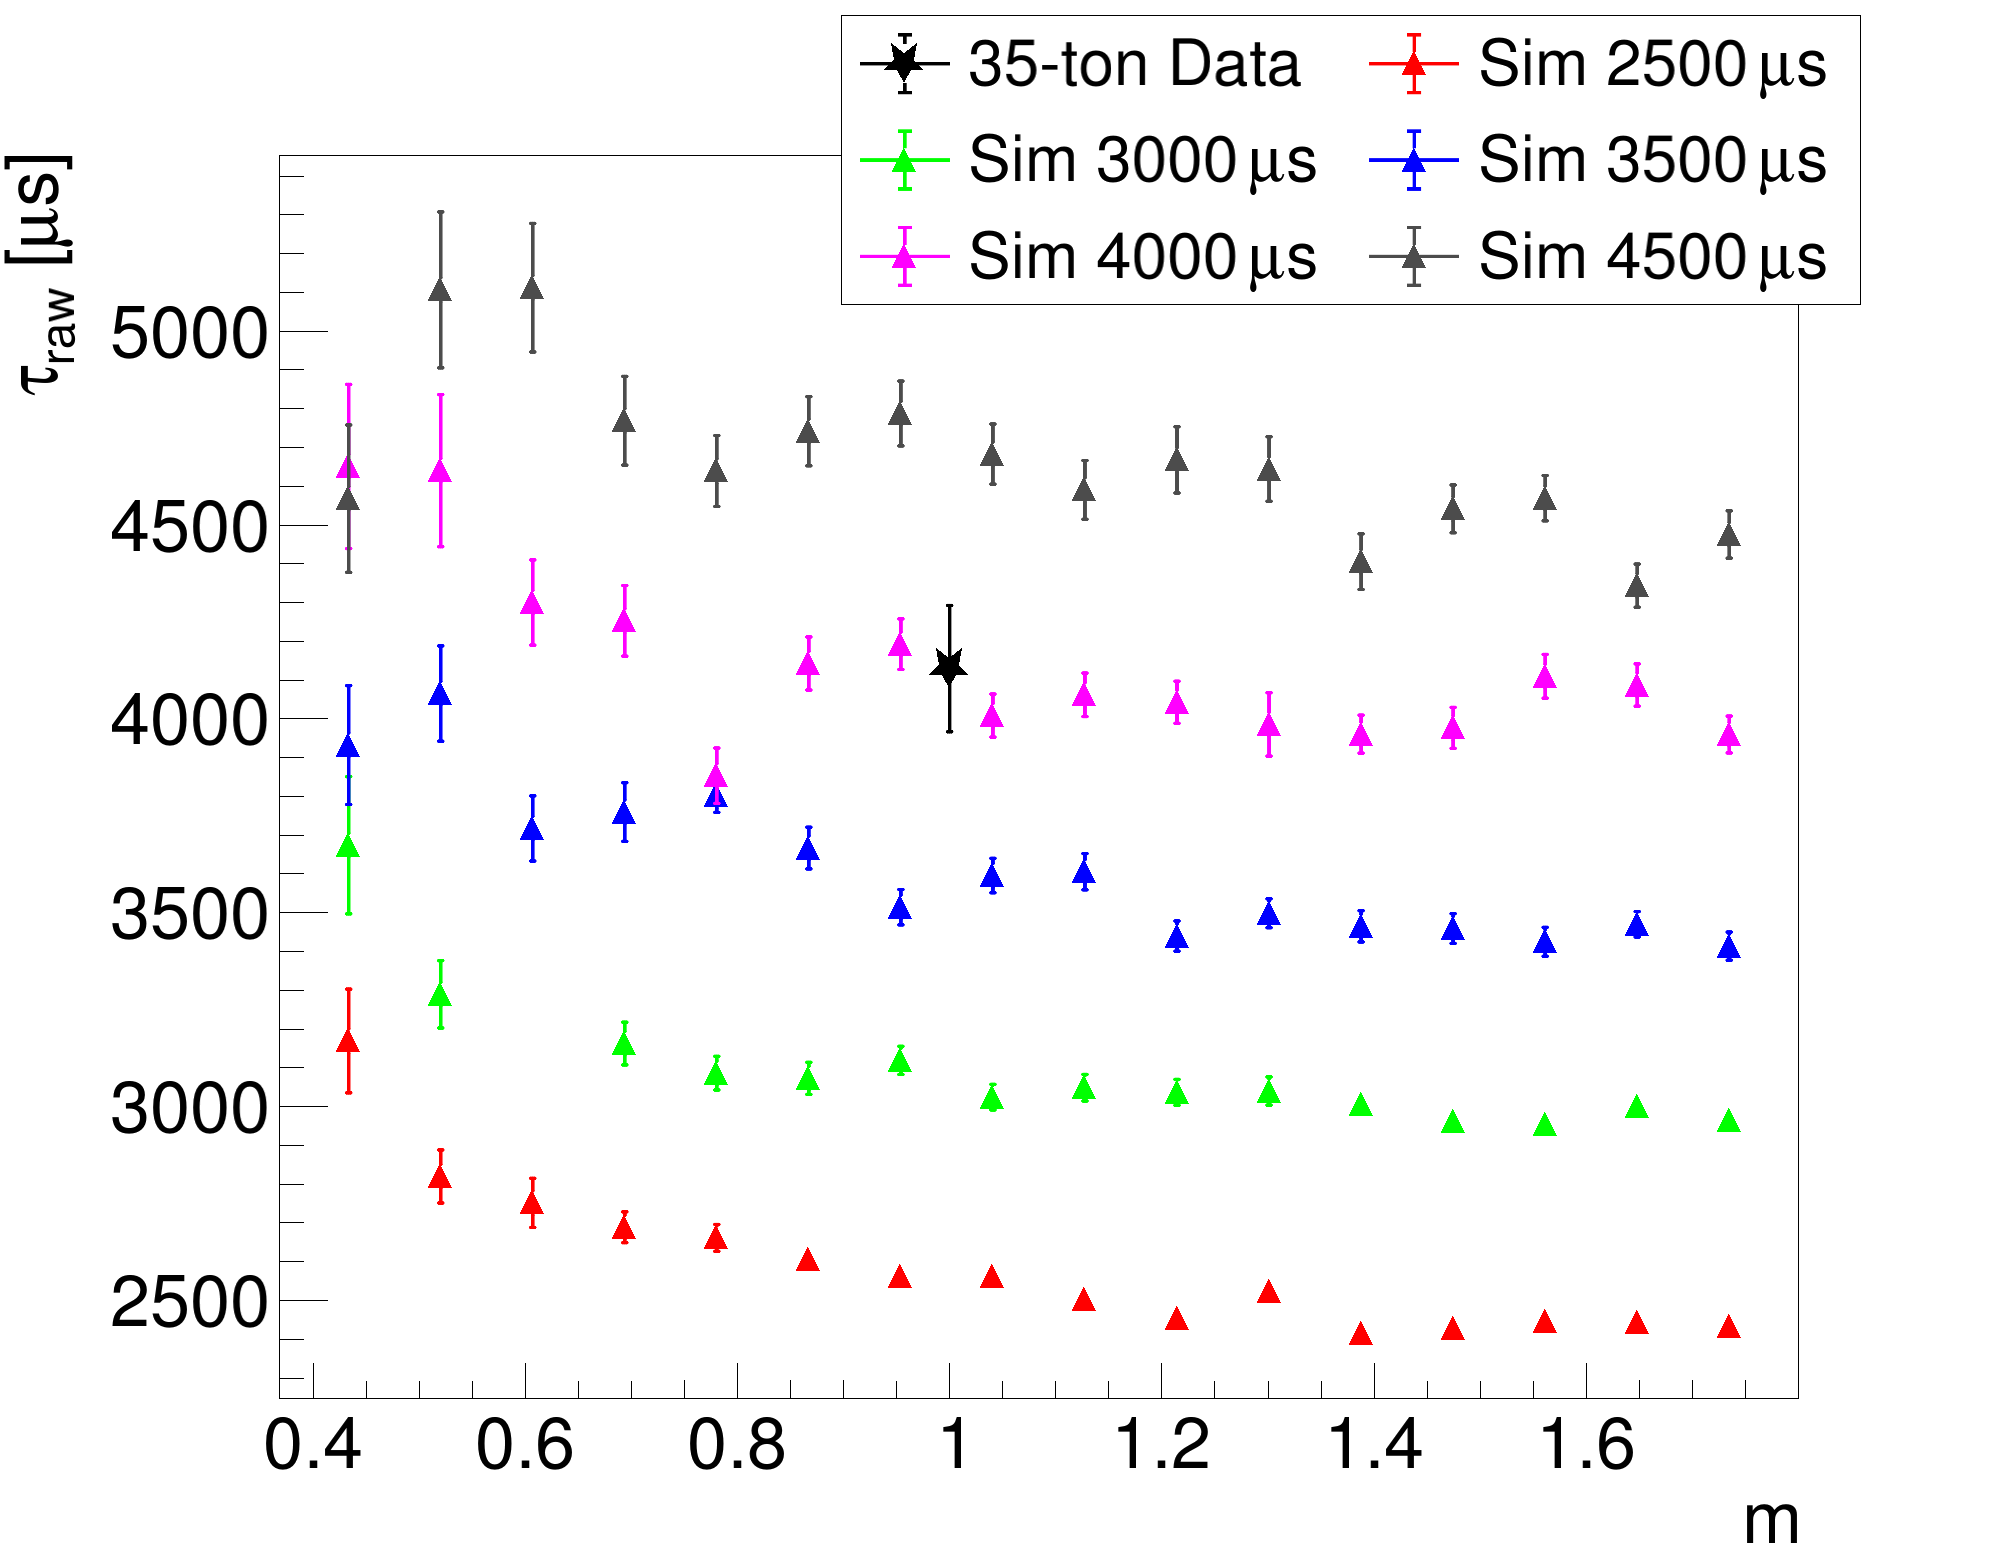
\includegraphics[width=\textwidth]{canvelifeVnoise.png}
\caption{$\tau_{\text{raw}}$ of simulated samples and 35-ton data.}
\label{fig:elifeVnoise}
\end{minipage}\hfill
\begin{minipage}[t]{0.48\textwidth}
\centering
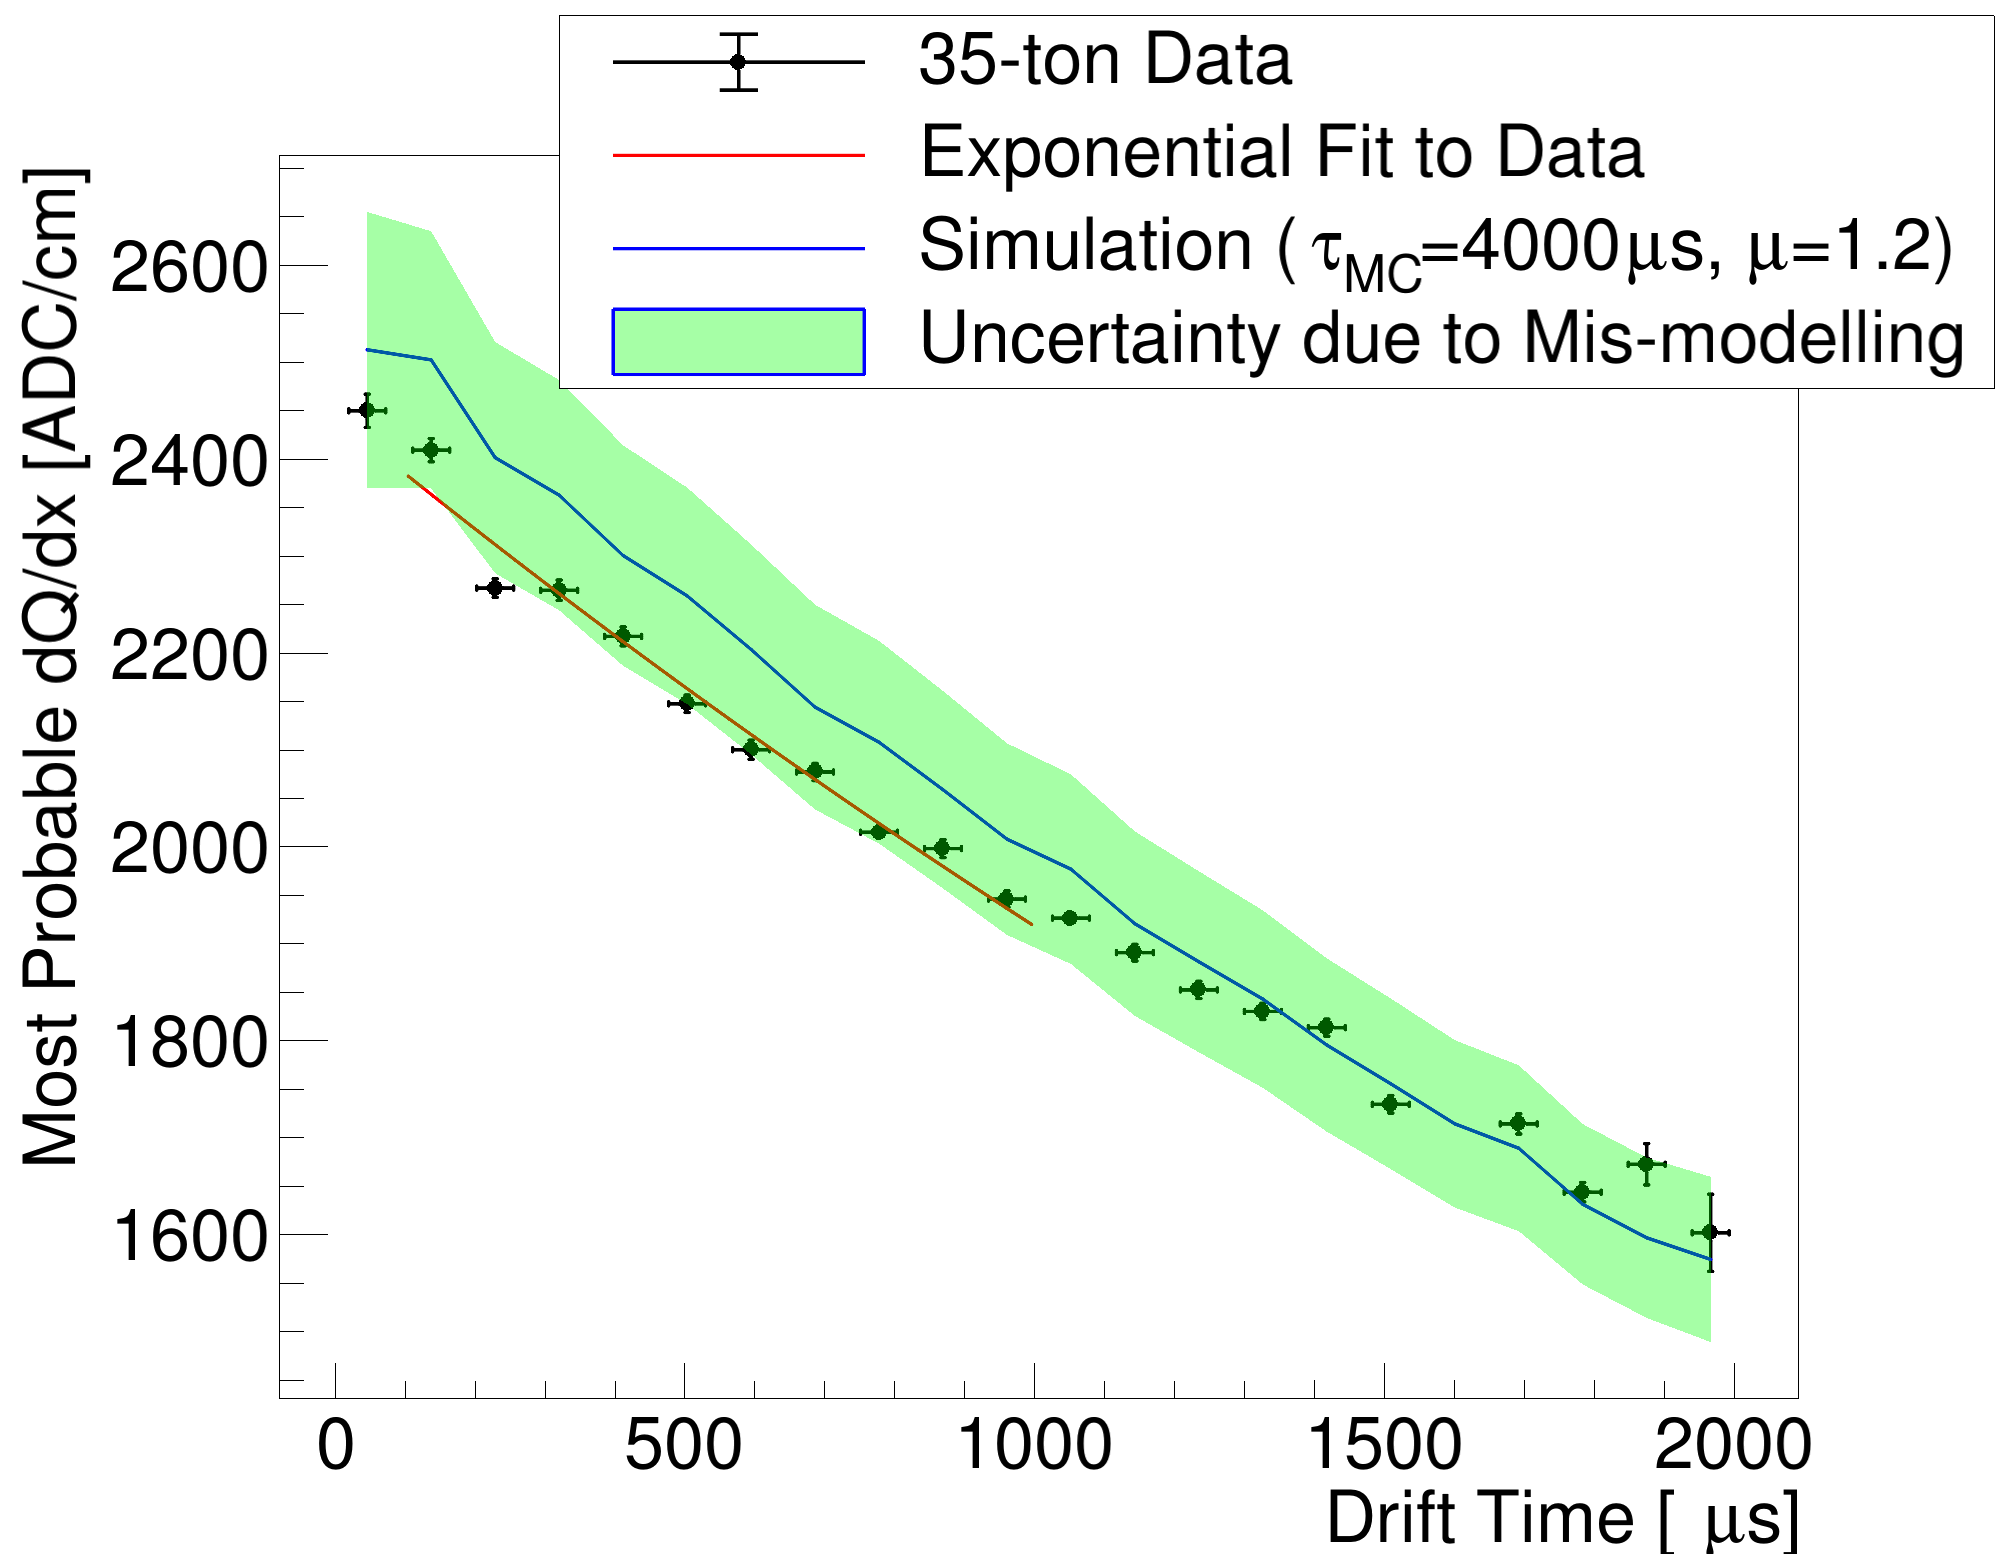
\includegraphics[width=\textwidth]{canvmpvpaper.png}
\caption{Data $dQ/dx$ MPV (black) overlaid with most similar simulated $dQ/dx$ MPV (blue). Green band represents the uncertainty due to $\mu$.}
\label{fig:mpvchoice}
\end{minipage}
\end{figure}

The corrected data electron lifetime is determined by performing a multivariate linear regression on the simulated sample results using the linear model
\begin{equation}\label{eq:lifetimecorrection}
\tau_{\text{corr},i} = \alpha_1 + \alpha_2 m_i + \alpha_3 \tau_{\text{raw},i} + \alpha_4 m_i\tau_{\text{raw},i} + \alpha_5 m_i^2 + \alpha_6 \tau_{\text{raw},i}^2
\end{equation}
for $i=1...n$ MC samples where $\tau_{\text{corr}}$ is the corrected electron lifetime (for MC, this is the true simulated lifetime, $\tau_{\text{MC}}$), $\tau_{\text{raw}}$ is the observed raw electron lifetime, and $m$ is the corrected $\mu$. The $\alpha$ coefficients are determined by performing the least squares regression on the matrix equation~\ref{eq:lifetimecorrection} for all $n=80$ MC samples where each $m=\mu/1.153$ is the reduced simulated $\mu$ relative to the data, which determines the correction factor between the observed lifetime and the true simulated lifetime. The data $\tau_{\text{corr}}$ is then determined by evaluating equation~\ref{eq:lifetimecorrection} using the data observed lifetime from figure~\ref{fig:landMPV}, $\tau_{\text{raw}}=4.24\pm0.10$~ms, $m=1.0$, and the coefficients determined using the MC samples. This process reveals the corrected lifetime for 35-ton data to be $\tau_{\text{corr}}=4.02\pm0.19$~ms.

\subsection{Systematic Uncertainties}\label{sec:lifetimesystematics}

The systematic uncertainty associated with the biases introduced by the noise is taken as the magnitude of the bias shift in the lifetime calculated in the previous section, $4.24-4.02=0.22$~ms, 5.5\%. This is assumed to account for the effects of low hit finding efficiency on the true Landau MPV, and the poor charge resolution for the relevant region of hit charge, both caused by the high level of noise in the detector.

Further uncertainty may be attributed to the accumulation of positive space charge in the TPC, which, because of their low mobility in comparison to the negative drift electrons, distorts the electric field~\cite{palestini}. Based on the nominal drift field of E$_0$=250~V/cm, the full drift distance of 2.2~m, and the rate of creation of positive ion density due to cosmic ray muons at the surface of the earth of about $1.8\times 10^{-10}$~C/m$^3$/s, the actual electric field becomes 0.89E$_0$ at the anode, and 1.19E$_0$ at the cathode. This overall field non-uniformity affects the probability of a drift electron to recombine with an argon ion. According to~\cite{argoneut-recombination}, the fraction of ionization electrons from a 1.8~MeV muon which survive recombination is 64.3\% in the absence of space charge, and 62.5\% at the anode and 66.7\% at the cathode with space charge distortions. This means a 4.2\% difference in available charge for drifting between the anode and cathode as a result of recombination alone. To determine the effect such a difference has on the decay lifetime we consider two exponential functions, $f(t)=Ae^{-t/\tau}$ and $g(t)=Ae^{-t/\tau'}$, which are equal-valued at $t=0$, $f(0)=g(0)$, and differ by a factor of $\alpha$ at $t=T$, $f(T)=(1+\alpha)g(T)$. Therefore, the lifetime parameter adjusted for space charge, $\tau'$, as a function of $\alpha$, is
\begin{equation}\label{eq:tauprime}
\tau'(\alpha) = \frac{T\tau}{T+\tau\log{(1+\alpha)}}.
\end{equation}
Thus, for this analysis ($\tau=4.02$~ms, $T\approx 2$~ms, and $\alpha=0.042$), the expected contribution of space charge distortions in electric field to the total systematic uncertainty of the electron lifetime to be 2.7\% for the fiducial region described in section~\ref{sec:fiducialcut}.

Other systematic differences between this measurement and the PrMs may be caused by inefficient mixing of impurities throughout the full cryostat volume. Previous internal computational fluid dynamics studies of the impurity mixing in the cryostat, taking into account fluid flow through the TPC field cage, suggest the possibility of at least a 10\% difference in the local LAr electron lifetimes between the location of PrM2 and within the TPC field cage~\cite{sdsu-cfd}. 

The measured lifetime of $4.02\pm0.19$~(stat.)~$\pm 0.25$~(syst.)~ms is marginally consistent with the average of the purity monitor measurements, $2.8\pm0.1$~(stat.)~$\pm0.5$~(syst.)~ms, over the same span of runs. 

\begin{thebibliography}{99}

\bibitem{MLESAC} P. H. S. Torr and A. Zisserman, ``MLESAC: A new robust estimator with application to estimating image geometry''. Computer Vision and Image Understanding. 78(1), 138-156. doi:10.1006/cviu.1999.0832 (1996).

\bibitem{CRY} C. Hagmann, D. Lange, and D. Wright, ``Cosmic-ray shower generator (CRY) for Monte Carlo transport codes''. 2007 IEEE Nuclear Science Symposium Conference Record. 2, 1143 (2007).

\bibitem{lifetimeT600} Amoruso, S., et al. (2004). "Analysis of the liquid argon purity in the ICARUS T600 TPC". Nucl. Instrum. Meth. A {\bf 516}, 68-79.

\bibitem{lifetime120L} arXiv:0910.5087v2

\bibitem{lifetimeT600_again} M.~Antonello {\it et al.},
  ``Experimental observation of an extremely high electron lifetime with the ICARUS-T600 LAr-TPC,''
  JINST {\bf 9}, no. 12, P12006 (2014)
  doi:10.1088/1748-0221/9/12/P12006
  [arXiv:1409.5592 [physics.ins-det]].
  
\bibitem{lifetime-argoneut} Anderson, C., et al. (2012). "The ArgoNeuT detector in the NuMI low-energy beam line at Fermilab". JINST {\bf 7}, P10019. arXiv:1205.6747

\bibitem{lifetime-longbo} Bromberg, C., et al. (2015). "Design and operation of LongBo: a 2~m long drift liquid argon TPC", JINST {\bf 10}, no. 07, P07015 (2015).
%. arXiv:1504.00398

\bibitem{baibussinov} baibussinov jinst 5 P03005

\bibitem{sdsu-cfd} Michna, G. J., Gent, S. P., and Propst, A. (2017). ``CFD Analysis of Fluid, Heat, and Impurity Flows in DUNE FAR Detector to Address Additional Design Considerations'', DUNE DocDB 3213.

\bibitem{palestini} Palestini, S., et al., ``Space charge in ionization detectors and the NA48 electromagnetic calorimeter'', Nucl. Instr. and Meth. A \textbf{421}, 75 (1999).

\bibitem{argoneut-recombination} Acciarri, R., et al. ``A study of electron recombination using highly ionizing particles in the ArgoNeuT Liquid Argon TPC''. JINST {\bf 8}, P08005 (2013).

\bibitem{dsp-book} Smith, S. W. ``The Scientist and Engineer's Guide to Digital Signal Processing''. California Technical Publishing, San Diego, CA, (1997). ISBN:0-9660176-3-3.

\end{thebibliography}

\end{document}